% ============================================================
%  main.tex  —  A Regime-Switching Framework for Tactical Sector Tilts
%  Preslav Vachev, emlyon business school, May 2026
% ============================================================
\documentclass[12pt, a4paper]{article}

% ── Packages ────────────────────────────────────────────────
\usepackage[T1]{fontenc}
\usepackage[utf8]{inputenc}
\usepackage{mathptmx}           % Times New Roman body + math
\usepackage[
  top=2.5cm, bottom=2.5cm,
  left=3.0cm, right=2.5cm
]{geometry}
\usepackage{setspace}
\usepackage{amsmath, amssymb}
\usepackage{graphicx}
\usepackage{booktabs}
\usepackage{multirow}
\usepackage{array}
\usepackage{longtable}
\usepackage{pdflscape}
\usepackage{tabularx}
\usepackage{xcolor}
\usepackage{soul}               % \hl{} highlighting
\usepackage{tcolorbox}          % fact-check boxes
\usepackage[hang, flushmargin]{footmisc}
\usepackage{caption}
\usepackage{float}
\usepackage{enumitem}
\usepackage{verbatim}
\usepackage{placeins}
\usepackage{fancyhdr}           % \FloatBarrier
\usepackage{titlesec}
\usepackage{parskip}
% bibliography handled manually in References section
\usepackage[
  colorlinks=true,
  linkcolor=black,
  citecolor=black,
  urlcolor=black
]{hyperref}

% ── Typography ───────────────────────────────────────────────
\onehalfspacing
\setlength{\parindent}{0pt}
\setlength{\parskip}{6pt}

% ── Section formatting ───────────────────────────────────────
\titleformat{\section}{\large\bfseries}{\thesection.}{0.5em}{}
\titleformat{\subsection}{\normalsize\bfseries}{\thesubsection}{0.5em}{}
\titlespacing*{\section}{0pt}{18pt}{6pt}
\titlespacing*{\subsection}{0pt}{12pt}{4pt}

% ── Fact-check box ───────────────────────────────────────────
\newtcolorbox{factcheck}{
  colback=yellow!20, colframe=red!60!black,
  fonttitle=\bfseries\small, title={\textcolor{red!70!black}{FACT-CHECK REQUIRED}},
  left=4pt, right=4pt, top=4pt, bottom=4pt, boxrule=0.8pt
}

% ── Figure/table placeholder ─────────────────────────────────
\newtcolorbox{placeholder}[1]{
  colback=blue!5, colframe=blue!40,
  fonttitle=\bfseries\small\color{blue!60!black},
  title={#1}, left=4pt, right=4pt, top=4pt, bottom=4pt,
  boxrule=0.6pt
}

% ── Caption style ────────────────────────────────────────────
\captionsetup{font=small, labelfont=bf, skip=4pt}

% ── Bibliography file ────────────────────────────────────────


% ============================================================
\begin{document}

% ── Footer ─────────────────────────────────────────────────────────────
\pagestyle{fancy}
\fancyhf{}
\renewcommand{\headrulewidth}{0pt}
\fancyfoot[C]{\small Vachev, P.}
\fancyfoot[R]{\small \thepage}
\fancypagestyle{plain}{%
  \fancyhf{}%
  \renewcommand{\headrulewidth}{0pt}%
  \fancyfoot[C]{\small Vachev, P.}%
  \fancyfoot[R]{\small \thepage}%
}


% ── Title page ──────────────────────────────────────────────
\begin{titlepage}
  \thispagestyle{empty}
  \centering
  \vspace*{2cm}
  {\small Vachev, P.\ --- Dissertation --- May 2026}\\[0.3cm]
  {\LARGE\bfseries A Regime-Switching Framework for Tactical Sector Tilts\\[0.4em]
   under Higher-Moment Investor Preferences}\\[2cm]
  {\large\itshape Preslav Vachev}\\[0.5cm]
  {\normalsize emlyon business school}\\[1.5cm]
  {\normalsize Supervisor: Professor Bertrand Tavin \quad|\quad May 2026}
  \vfill
\end{titlepage}
\pagenumbering{roman}

\clearpage
\begin{center}
  \vspace*{3cm}
  {\large\bfseries Acknowledgements}
\end{center}
\vspace{1.5cm}

\noindent
I would like to thank the emlyon faculty for inspiring a lasting interest in mathematical application.

\vspace{1cm}

\noindent
I would like to thank Professor Bertrand Tavin for his guidance and support throughout.

\vspace{1cm}

\noindent
I would also like to thank my mother, Palmina, for pushing me to pursue higher education abroad.

\clearpage

% ── Abstract ────────────────────────────────────────────────
\begin{abstract}
\noindent
This thesis develops and evaluates a regime-aware core-plus-satellite allocation framework
designed for implementation within the operational constraints of a wealth management context.
A three-state Hidden Markov Model is estimated on monthly excess log returns of the S\&P~500
Total Return index and the Bloomberg US Treasury 7--10 Year index. The resulting one-step-ahead
predictive regime probabilities serve as the signal for a scoring engine that evaluates nine US
sector ETFs and gold as candidate tilts against a 60/40 benchmark with a fixed 40\% Treasury allocation and a replaceable 60\% equity sleeve. Tilt scoring
follows a Taylor-expanded expected utility function after Jondeau and Rockinger (2006),
accommodating mean-variance, mean-variance-skewness, and mean-variance-kurtosis investor types.
The central design feature is a rolling 60-month estimation window that enables
the model to adapt to structural breaks in sector leadership, specifically the rotation from
energy sector dominance during the 2003--2008 commodity supercycle to technology sector
dominance in the post-2016 period. A score improvement floor functions as a hurdle rate,
returning the portfolio to the passive 60/40 core when regime conviction is insufficient.
The primary configuration (45\% satellite sleeve, score improvement floor = 0.001) achieves a CAGR of 8.60--8.90\% against a benchmark of 7.71\%, Sharpe ratios of 0.920--0.956 versus 0.875, and maximum drawdown improvements of approximately 335 basis points. A conservative 20\% sleeve variant is also reported, which simultaneously beats the benchmark on all five risk-adjusted metrics including downside deviation.
\end{abstract}

\vspace{6pt}
\noindent\textbf{Keywords:} Hidden Markov Model, regime switching, tactical asset allocation, sector rotation, higher-moment preferences, rolling window estimation, core-plus-satellite portfolio

\vspace{4pt}
\noindent\textbf{JEL Classification:} G11 (Portfolio Choice; Investment Decisions) $\cdot$ G17 (Financial Forecasting and Simulation) $\cdot$ C22 (Time-Series Models) $\cdot$ C61 (Optimization Techniques) $\cdot$ G23 (Pension Funds; Other Private Financial Institutions)

\newpage
\tableofcontents
\newpage
\pagenumbering{arabic}

\clearpage
% ============================================================
\clearpage
\section{Introduction}
% ============================================================

In the wealth management business, only a small percentage of clients are managed actively,
and that depends largely on the size and the cost of continuing operations of the firm. Most
individual clients and their portfolios are managed passively or on very infrequent rebalancing
schedules. These portfolios are usually standardised for several reasons: to facilitate the
communication chain between client, relationship manager, portfolio manager, and trading desk,
and to abide by rules and regulations.

Once a standardised approach has been developed for a firm, an operational pipeline follows,
with internal structures and processes built to maintain the order of business for smaller
clients. In recent years these processes have been optimised across the industry, but their
scale depends, again, on the size and cost of operations. According to PwC's Asset and Wealth
Management 2025 report, passive AUM is projected to reach USD~70 trillion by 2030 at an
annualised rate of 10\%, and 89\% of asset managers reported profitability pressure over the
five years preceding the report, with profit per AUM declining by approximately 19\% since 2018.
This is the operational economics argument that motivates the study: under cost pressure and
growing AUM, the practical default for smaller clients is a standardised passive mandate.

This poses the question at the core of this study: is it possible to develop a model with a
decision tilt that outperforms a passive benchmark on a risk-adjusted basis and that
simultaneously addresses the concerns of investors with different preferences for higher moments?
Most studies that use a regime switching framework to solve a portfolio allocation problem do so
considering different types of investors, but not the type of portfolio manager who operates
within a standardised, constrained mandate. This study deliberately caters to that audience.
The final version of the model developed here is designed for a wealth management context,
though it should not be excluded from other domains in the study of regime switching models,
portfolio allocation signals, and sector risk-return analysis.

The main empirical results are reported in \textbf{Table~\ref{tab:performance}}. We contribute to the regime-switching and portfolio allocation literature in several ways.
First, our regime-switching model is integrated within a rolling 60-month estimation window that
refits the HMM at every rebalance date, allowing the model to adapt to structural breaks in
sector leadership. Second, we introduce scoring for allocation decisions rather than solving an
optimisation problem, making the approach computationally manageable within a real operational
pipeline. Third, we incorporate multiple investor preference types, from mean-variance to
mean-variance-kurtosis, within the same framework, allowing the model to serve clients with
different attitudes toward tail risk. Finally, we integrate a score improvement floor that
functions as a hurdle rate, ensuring that the model only deviates from the passive core when
the regime signal provides sufficient expected utility justification.

The academic literature on asset allocation under regime switching was opened by
Ang and Bekaert (2002), who showed that the welfare cost of ignoring international
diversification is significantly amplified in bear regimes, particularly when a risk-free asset
is available. Ang and Bekaert (2004) subsequently demonstrated in a practitioner-oriented paper
that regime-based allocation strategies outperform static 60/40 even after transaction costs,
with the key insight being that the benefit comes from regime persistence rather than prediction.
Guidolin and Timmermann (2007, 2008) extended this framework to a four-state model and showed
that optimal allocations differ substantially across regimes and that ignoring regime switching
generates welfare costs of several cents per dollar of initial wealth at short investment
horizons, rising above eight cents at 60-month horizons under high risk aversion. The present
study sits in this tradition but departs from it in three important ways. We use a simpler,
operationally manageable scoring approach rather than full Bellman equation optimisation. We
focus on a US sector ETF universe rather than international equity. And we introduce rolling
window re-estimation as the mechanism for handling structural breaks, an aspect that was not
required in studies relying on the stable 1954--1999 data environment.

The thesis is structured as follows. Section~\ref{sec:litreview} reviews the relevant
literature. Section~\ref{sec:data} describes the data. Section~\ref{sec:model} presents
the Hidden Markov Model specification and estimation. Section~\ref{sec:preferences} develops
the investor preference theory and scoring function. Section~\ref{sec:allocation} describes
the allocation layer architecture. Section~\ref{sec:tilts} presents the satellite tilts,
conviction scalar, and rolling window mechanics. Section~\ref{sec:findings} reports the
key findings. Section~\ref{sec:gold} discusses gold as a conditional safe haven.
Section~\ref{sec:conclusion} concludes.

\clearpage
% ============================================================
\clearpage
\section{Literature Review}
\label{sec:litreview}
% ============================================================

\subsection{Regime Switching in Asset Allocation}

The regime-switching framework for financial time series originates with Hamilton (1989),
who introduced the Markov-switching model as a means of capturing structural change in
macroeconomic time series. Hamilton's key contribution was the filtered probability recursion,
which allows the latent state to be inferred from observed data using the EM algorithm,
producing a probabilistic assessment of the current regime rather than a binary classification.
This framework was subsequently extended to financial applications by a growing literature
documenting the presence of regimes in both stock and bond returns.

The first direct application to portfolio allocation under regime switching is Ang and
Bekaert (2002), who evaluate international asset allocation in the presence of bear and bull
regimes. Using a two-state HMM on international equity returns, they show that correlations
increase substantially during bear regimes, eroding the diversification benefit that static
mean-variance analysis predicts. The welfare cost of ignoring these regime-dependent
correlations is estimated at two to three cents per dollar of initial wealth when a
conditionally risk-free asset is included in the portfolio; in the all-equity case the cost
is substantially lower, at around 0.2 to 0.4 cents. They find that optimal portfolio weights
differ significantly across regimes. Ang and Bekaert (2004) extend this to a
practitioner-oriented study, demonstrating that regime-aware allocation strategies outperform
a static 60/40 benchmark even after transaction costs, with the key mechanism being regime
persistence: the model generates value because regimes last long enough for the allocation
signal to be actionable.

Guidolin and Timmermann (2007) provide the most comprehensive treatment of multivariate
regime switching for asset allocation, estimating a four-state model on US stocks and bonds
over 1954--1999 and solving the full dynamic programming problem for buy-and-hold and
rebalancing investors with power utility. Their four states, characterised as crash, slow
growth, bull, and recovery, exhibit very different means, volatilities, and cross-asset
correlations, and optimal allocations vary substantially across states. The welfare cost of
ignoring regimes is reported in cents per dollar of initial wealth (Table~5 of that paper),
reaching approximately eight cents at a 60-month horizon under high risk aversion. The paper
documents out-of-sample performance evaluation across multiple investor types and horizons
and finds that the regime model outperforms simpler benchmarks across most investment horizons.
A key finding relevant to the present study is that no VAR terms are required in the model,
suggesting that the return distribution itself, rather than predictive variables, carries the
relevant information. Guidolin and Timmermann (2008) extend this to international equity
markets, incorporating four-moment preferences and showing that regime switching generates
endogenous non-normality in portfolio returns, with co-skewness and co-kurtosis properties
playing an important role in home bias. The Ang and Timmermann (2012) survey subsequently
documents that multi-state specifications, generally three or more states, outperform two-state
models across a range of asset allocation applications, supporting the three-state specification
used in the present study.

The present study contributes to this literature in three specific ways. First, it applies the
HMM framework to the US sector ETF universe --- a dimension of the allocation problem that the
international equity focus of the preceding papers does not address. Second, it replaces the
full Bellman equation optimisation with a operationally manageable scoring approach, making the framework viable within a wealth management pipeline. Third, and most importantly,
it introduces a rolling 60-month estimation window as the mechanism for adapting to structural
breaks in sector leadership, explicitly addressing the stale-moment problem that arises when
an expanding window is used across multi-decade samples.

\subsection{Sector ETF Allocation under Regime Switching}

The application of regime switching to sector-level allocation is a relatively recent and
narrower strand of the literature. Ma, MacLean, Xu, and Zhao (2011) is the closest antecedent
to the present study, proposing a regime-dependent factor-risk-neutral strategy for the nine
State Street SPDR sector ETFs, the same universe used here. They model factor-risk-neutral
allocation using a Markov regime-switching framework and compare performance against an
equal-weight benchmark across the same ETF universe. Their results demonstrate that
regime-dependent sector allocation outperforms the static benchmark, and they use the same
sector ETF selection criteria applied here: the nine ETFs are from a single provider, have a
long trading history beginning December 1998, and provide comprehensive coverage of the US
market. The key difference between Ma et al.\ (2011) and the present study is that their
framework does not include a fixed bond core, does not incorporate higher-moment investor
preferences, and uses an expanding estimation window. The rolling window adaptation and the
core-plus-satellite architecture are specific contributions of the present study.

Dou, Gallagher, Schneider, and Walter (2014) provide direct empirical evidence that
cross-sector regime-dependent allocation outperforms cross-regional allocation on Sharpe ratio,
return, and beta in both in-sample and out-of-sample periods over 1995--2010. Their
unconstrained regime-switching sector strategy achieves an out-of-sample Sharpe ratio of 0.93
compared to 0.30 for the world market portfolio, with notably lower beta in bear regimes.
Under a benchmark constraint, the out-of-sample Sharpe narrows to 0.39 versus 0.32. Their
finding that sector allocation is more amenable to regime-based improvement than regional
allocation is consistent with the sector ETF focus of the present study, and their
documentation of lower cross-sector correlation during bear regimes supports the theoretical
motivation for the conviction scalar used in the allocation layer here. Jiang, Liu, and
Tse (2015) demonstrate similar results using international iShares ETFs with a daily
rebalancing MRS strategy, finding outperformance after transaction costs and providing
additional evidence that ETF-based regime switching strategies are practically implementable
at the institutional level.

\subsection{Higher-Moment Preferences and Taylor-Expanded Utility}

The theoretical foundation for incorporating skewness and kurtosis into investor preferences
is provided by Scott and Horvath (1980), who use proof by contradiction under the assumption
of decreasing absolute risk aversion to establish the sign of investor preference for moments
of higher order than variance. Their result that the third moment of the utility function is
positive (investors prefer positive skewness) and the fourth moment is negative (investors
dislike excess kurtosis) holds broadly for risk-averse utility functions, not just specific
parametric forms. This generality is important: it means the investor types defined in this
study do not depend on a specific assumed utility function, but on a universal property of
risk-averse behaviour.

Jondeau and Rockinger (2006) provide the operational implementation of these preferences
through a Taylor series expansion of expected utility around the moments of the return
distribution. Their four-moment approximation gives a closed-form scoring function that is
accurate for moderately non-normal distributions and that handles a large number of assets
without requiring the computationally prohibitive co-skewness and co-kurtosis tensors that
direct four-moment optimisation would require. A key finding in Jondeau and Rockinger (2006)
is that the opportunity cost of using only mean and variance to approximate expected utility
ranges from negligible in near-normal data environments to more than 25 cents per dollar in
highly non-normal settings such as emerging market or individual stock return distributions,
confirming that higher moments carry economically meaningful information when return
distributions are sufficiently non-normal. They also present and evaluate a full four-moment
MVSK investor who combines skewness preference and kurtosis aversion in a single objective
function. The present study deliberately separates these into distinct MVS and MVK investor
types, allowing the contribution of each moment to be isolated empirically. Kim, Fabozzi,
Cheridito, and Fox (2014) demonstrate that robust mean-variance portfolios implicitly favour
skewness and penalise kurtosis without requiring explicit higher-moment terms, providing a
complementary argument for the tractability of this approach.

\subsection{Rolling Window Estimation and Time-Varying Parameters}

The rolling window estimation approach used in this study is grounded in the parameter
instability literature. Pesaran and Timmermann (2007) establish that in the presence of
structural breaks, the optimal estimation window trades off bias from stale data against
variance from insufficient observations, and that rolling windows are preferred over expanding
windows when the data-generating process exhibits parameter instability. Their theoretical
results provide the formal justification for preferring a fixed-length rolling window over
the expanding window used in the earlier regime-switching literature. The Hematizadeh,
Tajaddini, and Hallahan (2022) time-varying transition probability study is also relevant:
their finding that even constant-transition-probability HMMs with rolling window estimation
capture most of the time-variation benefit of more complex TVTP models provides support for
the simpler constant-$P$ specification used here. Nystrup, Hansen, Madsen, and Lindstr{\"o}m
(2015) demonstrate that regime-based allocation with adaptive parameter estimation outperforms
static allocation without requiring return forecasting skill, with the key mechanism being
regime persistence rather than prediction accuracy. Their use of a confidence threshold before
changing positions is the conceptual antecedent of the score improvement floor mechanism in
the present study.

The rolling window specification in this study introduces a specific design tension worth
documenting in the literature. The number of states, $k=3$, is selected on the basis of the
full 27-year sample. The rolling 60-month estimation then uses this established structural
assumption to re-estimate only the parameter values within each window. This two-stage design
is analogous to model selection followed by rolling out-of-sample evaluation: the structural
form is validated on the full sample, and the rolling window then adapts the parameters of
that structure to the current data environment. The alternative of re-selecting $k$ at every
window would be computationally expensive, methodologically inconsistent, and likely to produce
spurious variation in the number of states that would interfere with the allocation signal.
The two-stage approach is both principled and practical, with one caveat: because $k=3$
is selected by inspecting the full sample that includes the evaluation period, this is a
modelling assumption rather than a fully out-of-sample structural choice. The rolling backtest
tests the performance of this fixed structural assumption under recursively updated parameters.

\clearpage
% ============================================================
\clearpage
\section{Data}
\label{sec:data}
% ============================================================

In order to define the regimes, one broad equity index and one broad bond index were used:
the S\&P~500 total return index and the Bloomberg US Treasury 7--10 Year index (LT09TRUU).
These monthly returns were continuously compounded. The S\&P~500 total return series was
obtained through the Yahoo Finance API, and the Bloomberg Treasury index through Bloomberg.
The 1-month T-Bill rate was subtracted from both to calculate the excess log return, which is
how both series are referred to in this study. The monthly T-Bill simple return was acquired
through the official Fama-French website and converted to log return for comparability with
the other data. The start of the sample period for constructing the HMM is January 1999 and
the end date is March 2026, matched to the issuance dates of the sector ETFs used for
satellite tilts.

For the satellite universe, this study uses the nine State Street SPDR sector ETFs: Materials
(XLB), Energy (XLE), Financials (XLF), Industrials (XLI), Technology (XLK), Consumer
Staples (XLP), Utilities (XLU), Health Care (XLV), and Consumer Discretionary (XLY). Gold
(XAU) is included as a tenth satellite candidate. All nine sector ETF return series were obtained through the Yahoo Finance API. The gold (XAU) return series was obtained from Bloomberg.

The selection of LT09TRUU as the bond component of the regime identification model was made
after comparing three bond index variants: the Bloomberg US Aggregate Bond Index (LBUSTRUU),
the Bloomberg US Treasury 7--10 Year index (LT09TRUU), and a mutual fund proxy tracking the
Aggregate index (WFBIX). The Treasury-only index produced the most economically interpretable
and stable regimes, particularly across the 2001 dotcom crash, the 2008 Global Financial
Crisis, and the 2020 COVID-19 period. This is consistent with the intuition that a
pure-rate-risk instrument with no credit exposure provides a cleaner signal for the
bond-equity correlation dynamics that drive regime identification.

During the exploration phase of this project, monthly data from the EURUSD exchange rate,
WTI crude oil, and bond indices at alternative durations were also tested with the Hidden
Markov Model. Those outputs were either too noisy or could not be realistically interpreted
in a macroeconomic context. Given the focus of the study on sector ETF tilts, their inclusion
could not be reasonably justified at this stage of the research.



\textbf{Figure~\ref{fig:price_levels}} shows the full price history of all twelve assets. Together, the S\&P~500 TR and LT09TRUU constitute the 60/40 benchmark core at a
fixed weight allocation. The choice of a 60/40 split is the industry standard for a balanced
client mandate and represents the passive baseline against which all strategy configurations
are evaluated.

\paragraph*{Rebalancing timeline and data construction.} All series are monthly end-of-month log returns from total-return adjusted prices. Bloomberg indices are total-return series. The no-look-ahead convention is strict: the HMM is estimated using returns through month $t$; predictive probabilities $\boldsymbol{\pi}_{t+1|t}$ are computed from the filtered state at $t$; weights are set at the close of month $t$ and earn returns in month $t+1$. Transaction costs of 5 basis points per side are deducted at rebalancing. The risk-free rate is aligned to the same month-end.

\begin{figure}[htbp]
  \centering
  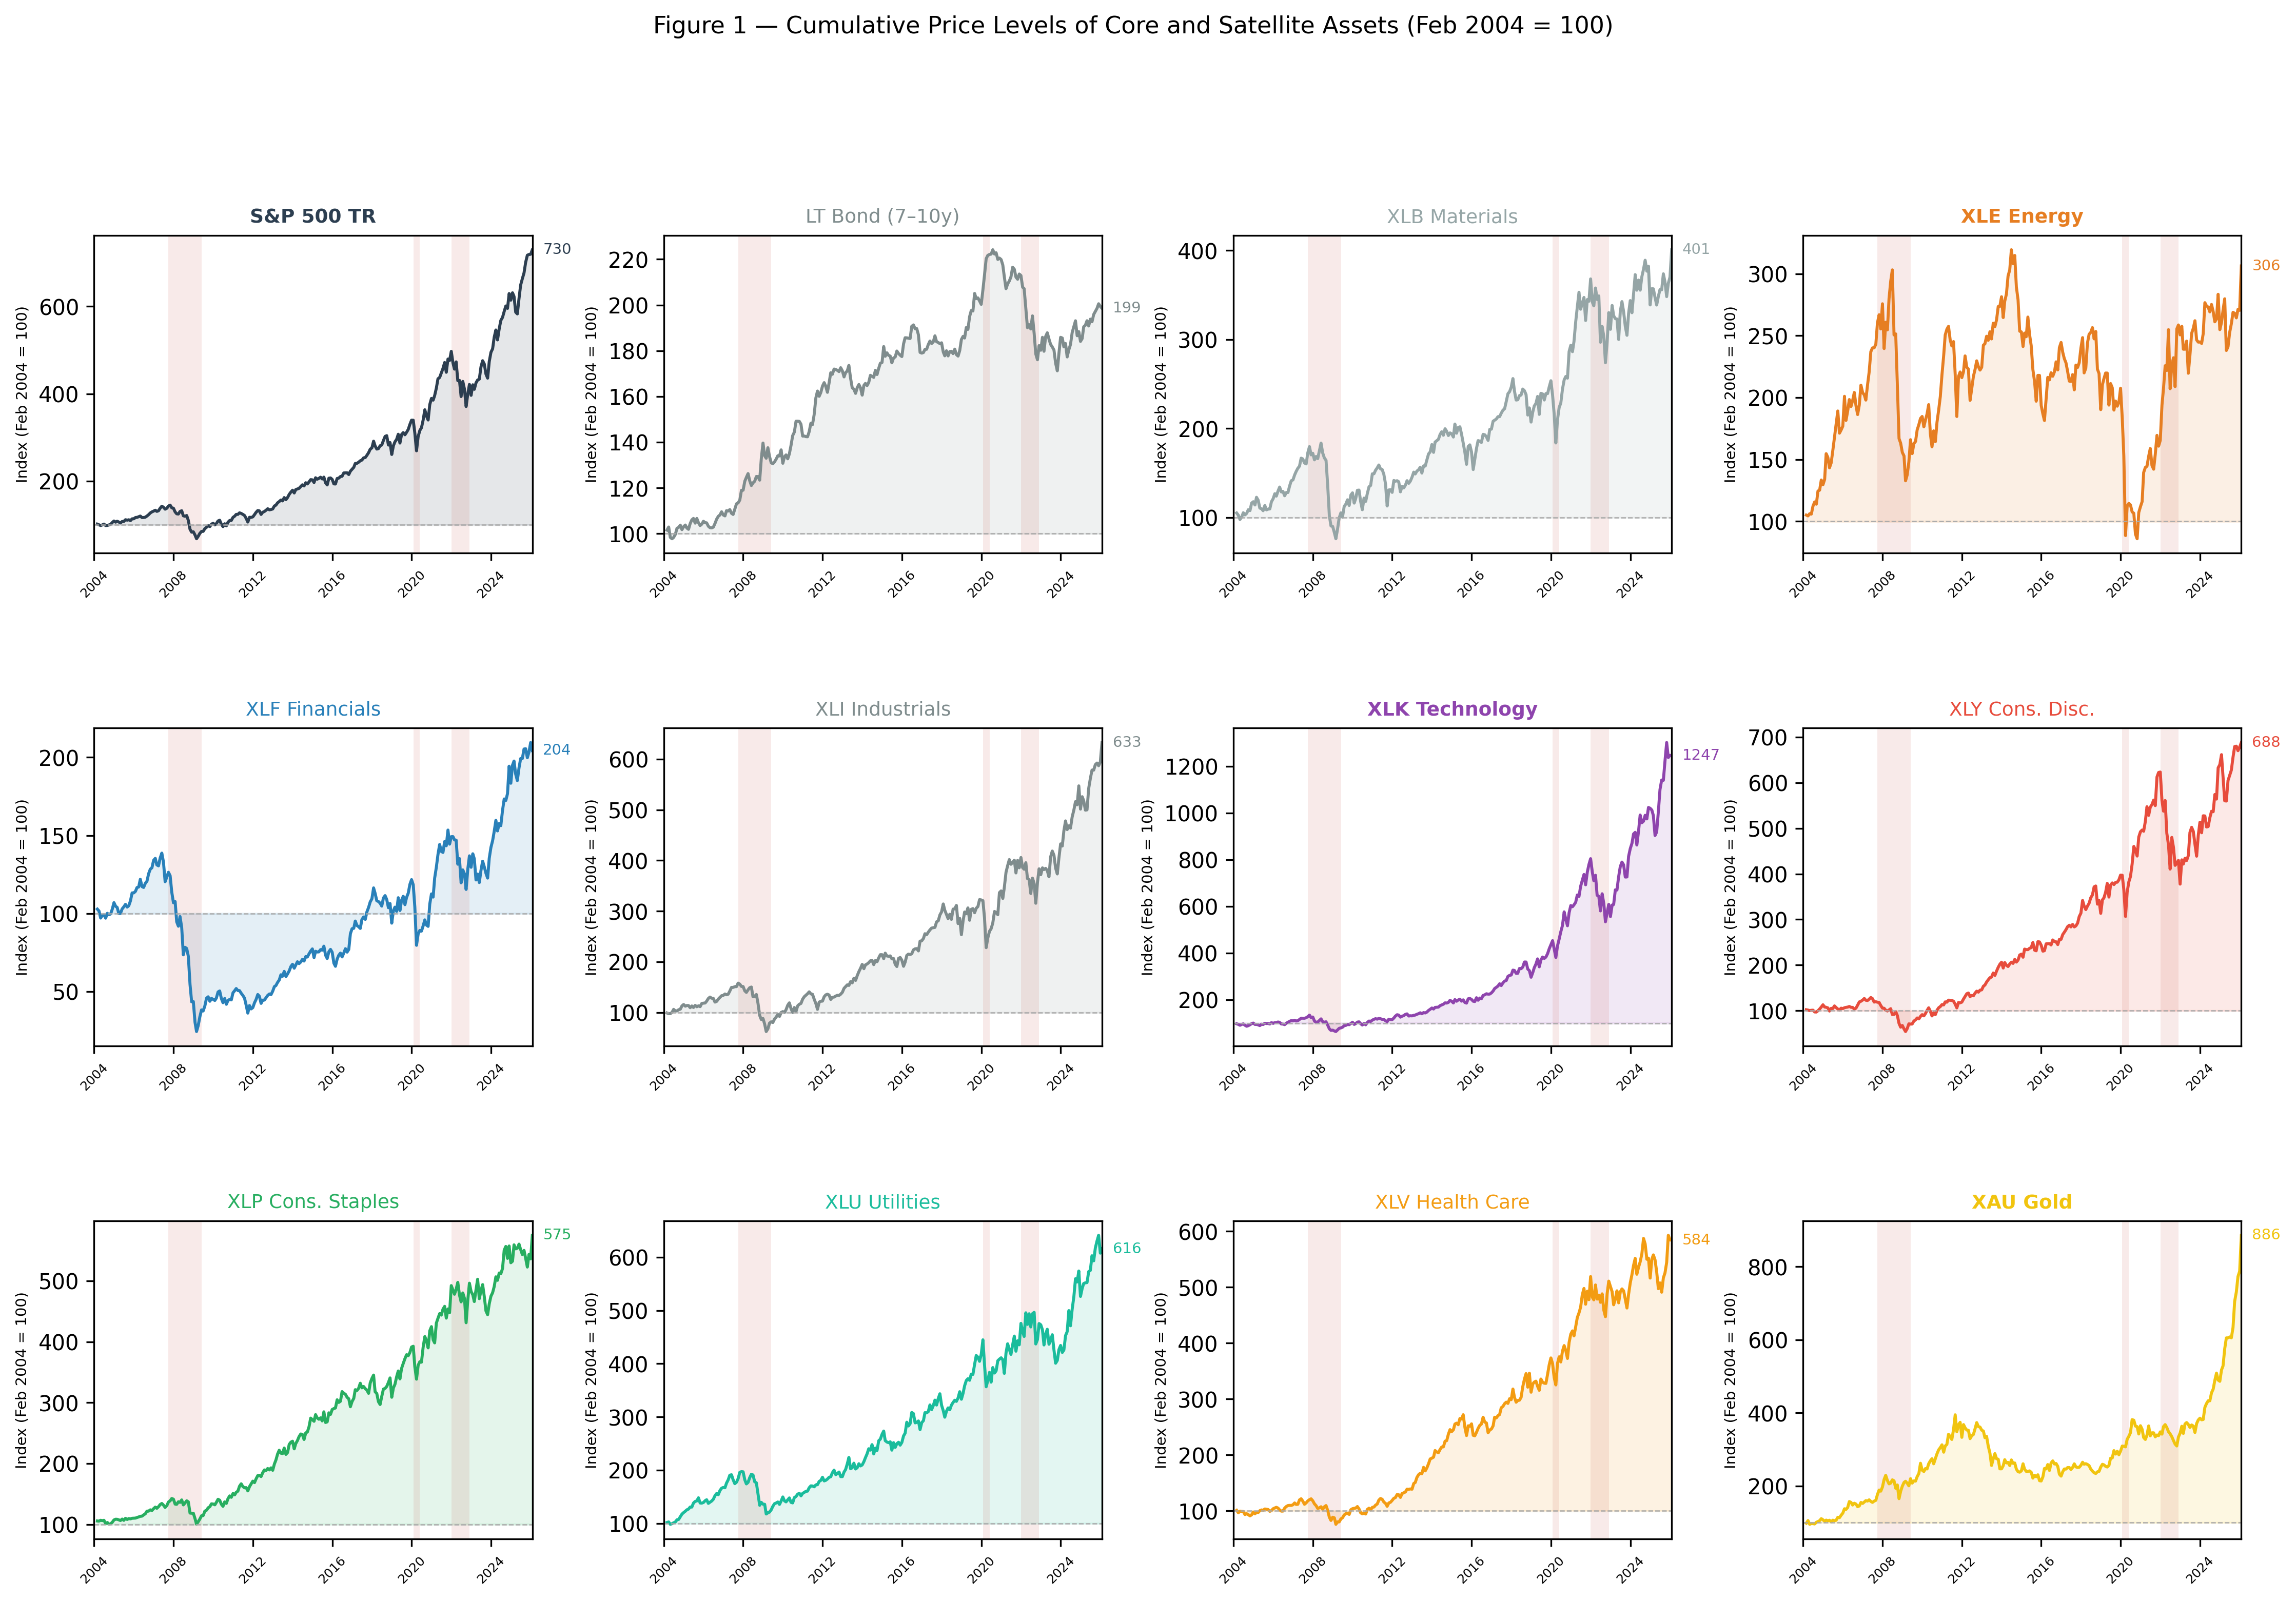
\includegraphics[width=\linewidth, height=0.52\textheight, keepaspectratio]{figures/fig1_asset_price_levels}
  \caption{Cumulative price levels of the core and satellite assets, rebased to 100 at
           February 2004. Shaded regions mark the four crisis episodes. Final index values
           are annotated at the right of each panel. XLK (Technology, 1247) and XAU
           (Gold, 896) are the highest-returning satellites over the full period;
           XLE (Energy, 306) and XLF (Financials, 204) are the weakest cyclical performers,
           reflecting the post-2014 energy bear market and the persistent post-GFC
           underperformance of financials respectively.}
  \label{fig:price_levels}
\end{figure}

\clearpage
% ============================================================



\begin{table}[H]
\centering
\caption{Descriptive Statistics for Monthly Log Returns --- Full Sample (Feb 2004 -- Jan 2026)}
\label{tab:data_stats}
\setlength{\tabcolsep}{4pt}
\footnotesize
\resizebox{\textwidth}{!}{%
\begin{tabular}{lrrrrrrr}
\toprule
\textbf{Asset} & \textbf{Ann.\ Mean (\%)} & \textbf{Ann.\ Vol (\%)} & \textbf{Sharpe} & \textbf{Skewness} & \textbf{Exc.\ Kurt.} & \textbf{Min (\%)} & \textbf{Max (\%)} \\
\midrule
\multicolumn{8}{l}{\textit{Core assets}} \\[2pt]
S\&P 500 TR        & 10.16 & 14.65 & 0.523 & $-$0.806 & 1.831 & $-$18.39 & 12.06 \\
LT Bond (7--10y)   &  3.33 &  6.41 & 0.129 & \phantom{$-$}0.056 & 0.868 & $-$4.80  & 7.69  \\
\midrule
\multicolumn{8}{l}{\textit{Cyclical sector satellites}} \\[2pt]
XLB Materials      &  8.32 & 19.77 & 0.294 & $-$0.567 & 1.842 & $-$25.35 & 15.99 \\
XLE Energy         &  8.63 & 25.99 & 0.236 & $-$0.667 & 4.539 & $-$42.12 & 26.82 \\
XLF Financials     &  5.72 & 21.67 & 0.149 & $-$1.120 & 4.116 & $-$30.38 & 19.72 \\
XLI Industrials    & 10.12 & 18.30 & 0.417 & $-$0.733 & 2.334 & $-$20.61 & 16.61 \\
XLK Technology     & 13.14 & 17.92 & 0.594 & $-$0.485 & 0.376 & $-$17.58 & 12.87 \\
XLY Cons.\ Disc.   & 10.52 & 18.53 & 0.433 & $-$0.257 & 1.415 & $-$19.40 & 17.30 \\
\midrule
\multicolumn{8}{l}{\textit{Defensive sector satellites}} \\[2pt]
XLP Cons.\ Staples &  8.66 & 11.69 & 0.527 & $-$0.578 & 1.168 & $-$13.48 & 9.94  \\
XLU Utilities      &  9.31 & 14.21 & 0.479 & $-$0.848 & 1.020 & $-$13.93 & 10.03 \\
XLV Health Care    &  8.98 & 13.62 & 0.476 & $-$0.379 & 0.449 & $-$13.23 & 11.86 \\
\midrule
\multicolumn{8}{l}{\textit{Commodity satellite}} \\[2pt]
XAU Gold           & 11.36 & 16.75 & 0.529 & $-$0.184 & 0.621 & $-$18.50 & 12.49 \\
\bottomrule
\end{tabular}}
\begin{minipage}{\linewidth}
\vspace{4pt}\footnotesize
\textit{Notes:} Monthly log returns from the allocation backtest period (February 2004 -- January 2026, $T=264$ monthly observations). Annual mean and volatility obtained by multiplying monthly mean by 12 and monthly standard deviation by $\sqrt{12}$. Sharpe ratio uses an approximate average 1-month T-bill rate of 2.5\% per annum as the risk-free rate. Skewness and excess kurtosis use Fisher's definition. All nine sector ETF returns obtained via Yahoo Finance API; XAU obtained from Bloomberg; LT Bond = \texttt{LT09TRUU} Bloomberg US Treasury 7--10 Year index.
\end{minipage}
\end{table}


\begin{table}[H]
\centering
\caption{Pairwise Correlation Matrix of Monthly Log Returns (Feb 2004 -- Jan 2026)}
\label{tab:correlations}
\setlength{\tabcolsep}{3.5pt}
\footnotesize
\resizebox{\textwidth}{!}{%
\begin{tabular}{lrrrrrrrrrrrr}
\toprule
 & \textbf{SP500} & \textbf{Bond} & \textbf{XLB} & \textbf{XLE} & \textbf{XLF} & \textbf{XLI} & \textbf{XLK} & \textbf{XLY} & \textbf{XLP} & \textbf{XLU} & \textbf{XLV} & \textbf{XAU} \\
\midrule
SP500 & 1.00 & $-$0.06 & 0.86 & 0.63 & 0.85 & 0.92 & 0.90 & 0.90 & 0.72 & 0.51 & 0.75 & 0.09 \\
Bond  &      & 1.00 & $-$0.11 & $-$0.25 & $-$0.16 & $-$0.11 & $-$0.03 & $-$0.03 & 0.10 & 0.22 & 0.04 & 0.32 \\
XLB   &      &      & 1.00 & 0.68 & 0.75 & 0.87 & 0.71 & 0.77 & 0.63 & 0.43 & 0.65 & 0.24 \\
XLE   &      &      &      & 1.00 & 0.55 & 0.63 & 0.46 & 0.48 & 0.42 & 0.33 & 0.43 & 0.13 \\
XLF   &      &      &      &      & 1.00 & 0.84 & 0.63 & 0.75 & 0.59 & 0.34 & 0.62 & $-$0.03 \\
XLI   &      &      &      &      &      & 1.00 & 0.76 & 0.83 & 0.69 & 0.45 & 0.66 & 0.06 \\
XLK   &      &      &      &      &      &      & 1.00 & 0.83 & 0.55 & 0.40 & 0.58 & 0.04 \\
XLY   &      &      &      &      &      &      &      & 1.00 & 0.59 & 0.36 & 0.61 & 0.03 \\
XLP   &      &      &      &      &      &      &      &      & 1.00 & 0.60 & 0.68 & 0.13 \\
XLU   &      &      &      &      &      &      &      &      &      & 1.00 & 0.46 & 0.23 \\
XLV   &      &      &      &      &      &      &      &      &      &      & 1.00 & 0.10 \\
XAU   &      &      &      &      &      &      &      &      &      &      &      & 1.00 \\
\bottomrule
\end{tabular}}
\begin{minipage}{\linewidth}
\vspace{4pt}\footnotesize
\textit{Notes:} Pearson correlations of monthly log returns. Several features of this matrix motivate the satellite selection logic. XAU (gold) has near-zero correlation with all sector ETFs and a mildly negative correlation with bonds, confirming its role as a diversifier orthogonal to both core assets. XLE (energy) has the lowest correlation with the S\&P~500 among cyclical sectors (0.63), explaining its frequent selection during the 2004--2009 commodity supercycle. XLU (utilities) has the lowest sector-to-S\&P~500 correlation (0.51) among the cyclicals, consistent with its defensive classification. Bond--equity correlation is $-0.06$ unconditionally but varies substantially across regimes, as documented in \textbf{Table~\ref{tab:summary_stats}}.
\end{minipage}
\end{table}

\clearpage
\section{Model}
\label{sec:model}
% ============================================================

There are several criteria that predate the use of a HMM and are specific to this study.
The outputs of the model need to have an intuitive economic interpretation that can be
communicated to a portfolio manager, where we assume the portfolio manager is familiar with
the concepts of expected return, standard deviation, and correlation, and understands their
interpretation in a portfolio context. The identified regimes need to be stable across seeds
and sample periods in order to reliably recognise key global events such as the dotcom crash,
the Global Financial Crisis, and the COVID-19 pandemic. The outputs need to serve as input
signals to the allocation layer. And the covariance between assets needs to be conditional
on the regime, in order to capture the co-movement dynamics that inform the satellite tilt
selection.

An important design point concerns what variables are used to define the regimes. This model
is entirely endogenous: the regimes are identified exclusively from the joint distribution
of the two return series, with no dividend yield, short-term interest rates, or
macroeconomic variables introduced as exogenous predictors. This stands in contrast to a
number of papers in the regime-switching literature, including the VAR-extended specification
of Guidolin and Timmermann (2007) and the macro-conditioned models in the time-varying
transition probability literature, which introduce external conditioning variables to capture
predictability beyond the return distribution itself. The choice of an endogenous
specification here is deliberate: it keeps the model self-contained within the information
available from traded prices alone, which is consistent with the operational context of a
wealth management firm that may not have reliable real-time macro feeds at the frequency and
latency required for monthly rebalancing.

Regime-switching models for financial time series belong to a broader family of models that
include threshold autoregressive models, hidden Markov models, hidden semi-Markov models,
and smooth-transition models. Within this family, the Hidden Markov Model with Gaussian
emissions was selected because it satisfies all four criteria above and because its filtered
probability output is directly usable as a forward-looking allocation signal without
additional transformation. GARCH-family models are widely used in the literature on
co-movement and conditional heteroskedasticity, and this family of models produces valuable
insights into the time-varying second moment structure of returns. However, GARCH outputs do
not naturally produce discrete regime labels that partition the joint return distribution
into economically interpretable states, which is a specific requirement of the allocation
layer in this study. The HMM's filtered probabilities, by contrast, provide a direct
probability distribution over a small number of interpretable states at each point in time.

\subsection{HMM Specification}

Let $\mathbf{Y}_t = (y_{1t},\, y_{2t})^{\prime}$ denote the bivariate vector of monthly
excess log returns on the S\&P~500 Total Return index and LT09TRUU at time
$t = 1,\ldots,T$. The Hidden Markov Model assumes that the conditional distribution of
$\mathbf{Y}_t$ is governed by an unobservable discrete state variable $S_t$ that takes
values in $\{0,1,\ldots,K-1\}$ and follows a first-order Markov chain with constant
transition probability matrix $\mathbf{P}$, where element
$p_{ij} = \Pr(S_{t+1}=j \mid S_t=i)$.

Conditional on the state, returns are assumed to follow a multivariate normal distribution:
\begin{equation}
  \mathbf{Y}_t \mid S_t = k \;\sim\; \mathcal{N}\!\left(\boldsymbol{\mu}_k,\,
  \boldsymbol{\Sigma}_k\right)
  \label{eq:hmm_emission}
\end{equation}
where $\boldsymbol{\mu}_k$ is the $(2\times 1)$ vector of state-conditional mean excess
returns and $\boldsymbol{\Sigma}_k$ is the $(2\times 2)$ full covariance matrix for state
$k$. The full covariance specification is essential: it allows the model to capture both
state-specific volatility and state-specific cross-asset correlations, which are the
mechanism through which the model captures regime-dependent bond-equity co-movement.
As shown in \textbf{Table~\ref{tab:summary_stats}}, this correlation varies substantially
across regimes and does not follow a simple negative-in-bear pattern.

The initial state distribution is parameterised as
$\boldsymbol{\pi}_0 = (\pi_{0,0},\ldots,\pi_{0,K-1})^{\prime}$ and estimated alongside the
other parameters. The full parameter vector is
$\boldsymbol{\theta} = \{\boldsymbol{\mu}_k, \boldsymbol{\Sigma}_k, \mathbf{P},
\boldsymbol{\pi}_0\}_{k=0}^{K-1}$.

\subsection{Estimation}

The model is estimated by maximum likelihood via the Expectation-Maximisation algorithm
introduced by Hamilton (1989). The implementation uses the \texttt{hmmlearn} Python library,
with custom pre-processing for excess log return construction and post-processing for regime
ordering and rolling window management. The EM algorithm iterates between two steps. The
E-step computes the filtered state probabilities using the Hamilton filter:
\begin{equation}
  \xi_{t|t}(k) = \Pr\!\left(S_t = k \mid \mathbf{Y}_1,\ldots,\mathbf{Y}_t;\,
  \boldsymbol{\theta}\right)
  \label{eq:filtered}
\end{equation}
These filtered probabilities are the forward-pass output of the filter: they represent the
probability of being in regime $k$ given all information available up to and including
time $t$. They are computed recursively from the prediction step:
\begin{equation}
  \xi_{t|t-1}(k) = \sum_{j} \xi_{t-1|t-1}(j)\, p_{jk}
  \label{eq:prediction}
\end{equation}
updated with the likelihood of the current observation in each state.

The M-step updates $\boldsymbol{\theta}$ by maximising the expected complete-data
log-likelihood with respect to the smoothed state probabilities. Convergence is declared
when the improvement in log-likelihood between iterations falls below $10^{-6}$. To mitigate
the risk of converging to local optima, 25 random initialisations were run and the solution
with the highest converged log-likelihood was retained.

\paragraph*{Likelihood computation via the forward algorithm.}

The observed-data log-likelihood is obtained by integrating out the latent state sequence.
For a single observation $\mathbf{Y}_t$ in state $k$, the state-conditional emission density is:
\begin{equation}
  f(\mathbf{Y}_t \mid S_t = k;\,\boldsymbol{\theta})
  = \frac{1}{(2\pi)^{n/2}\,|\boldsymbol{\Sigma}_k|^{1/2}}
    \exp\!\left(-\tfrac{1}{2}
    (\mathbf{Y}_t - \boldsymbol{\mu}_k)^\prime
    \boldsymbol{\Sigma}_k^{-1}
    (\mathbf{Y}_t - \boldsymbol{\mu}_k)
    \right)
  \label{eq:emission_density}
\end{equation}
where $n = 2$ is the number of observed series. The full observed-data log-likelihood
$\mathcal{L}(\boldsymbol{\theta}) = \log p(\mathbf{Y}_1,\ldots,\mathbf{Y}_T;\,\boldsymbol{\theta})$
is evaluated using the forward (filter) recursion. Define the forward variable:
\begin{equation}
  \alpha_t(k) = p(\mathbf{Y}_1,\ldots,\mathbf{Y}_t,\, S_t = k;\,\boldsymbol{\theta})
  \label{eq:forward_var}
\end{equation}
The recursion is initialised at $t = 1$ as:
\begin{equation}
  \alpha_1(k) = \pi_{0,k} \cdot f(\mathbf{Y}_1 \mid S_1 = k;\,\boldsymbol{\theta})
\end{equation}
and propagated forward for $t = 2,\ldots,T$:
\begin{equation}
  \alpha_t(k) = f(\mathbf{Y}_t \mid S_t = k;\,\boldsymbol{\theta})
                \sum_{j=0}^{K-1} \alpha_{t-1}(j)\, p_{jk}
  \label{eq:forward_recursion}
\end{equation}
The log-likelihood is then:
\begin{equation}
  \mathcal{L}(\boldsymbol{\theta})
  = \sum_{t=1}^{T} \log \sum_{k=0}^{K-1} \alpha_t(k)
  \label{eq:loglik}
\end{equation}
In practice, the recursion is implemented in log-space using the log-sum-exp trick to avoid
numerical underflow, which is the approach taken in \texttt{hmmlearn}. The filtered
probabilities from Equation~\eqref{eq:filtered} are recovered by normalising:
$\xi_{t|t}(k) = \alpha_t(k) \,/\, \sum_j \alpha_t(j)$.

The following code illustrates the core estimation call. \texttt{GaussianHMM} from \texttt{hmmlearn} is used with \texttt{covariance\_type="full"} to allow a distinct full covariance matrix per regime. Twenty-five random initialisations are run and the best log-likelihood solution is retained.

\begin{verbatim}
from hmmlearn import hmm
import numpy as np

best_model, best_ll = None, -np.inf

for seed in range(1, 26):
    model = hmm.GaussianHMM(
        n_components=3,
        covariance_type="full",
        n_iter=2000,
        tol=1e-6,
        random_state=seed,
    )
    model.fit(X)           # X: (T, 2) array of excess log returns
    ll = model.score(X)
    if ll > best_ll:
        best_ll, best_model = ll, model

# One-step-ahead predictive probabilities
filtered    = best_model.predict_proba(X)
predictive  = filtered @ best_model.transmat_
\end{verbatim}

Post-estimation, regimes are reordered by ascending mean equity return so that Regime~0 is always the bear state, consistently across all seeds and rolling windows.


\subsection{Model Selection and the Two-Stage Design Rationale}

Three state configurations were evaluated: $K=2$, $K=3$, and $K=5$. The two-state model
collapsed the bear and transitional periods into a single high-volatility state, losing the
distinction between genuine market stress and regime uncertainty. The five-state model
produced average regime durations of one to two months with no stable economic interpretation,
consistent with the overfitting behaviour documented in Guidolin and Timmermann (2007).
The three-state model, $K=3$, produced economically interpretable and statistically stable
regimes across the full sample.

It is important to explain the two-stage nature of this design, as a potential
methodological concern arises from the fact that $k=3$ was selected by examining the full
27-year sample, while the actual allocation strategy uses a rolling 60-month estimation
window. These are two separate and complementary uses of the model. The full-sample
estimation is a diagnostic exercise: its purpose is to establish that three states are the
appropriate structural assumption for this asset pair, that these states are stable enough
to carry economic interpretation, and that they recur across multiple market cycles in a
consistent way. This is the model selection stage. Once $k=3$ is established as the correct
structural assumption, the rolling window then takes this as given and re-estimates only the
parameter values, not the number of states, within each 60-month window.

\begin{table}[htbp]
\centering
\caption{Model Selection: Log-Likelihood, AIC and BIC for $K = 2, 3, 5$ States}
\label{tab:model_selection}
\setlength{\tabcolsep}{8pt}
\small
\begin{tabular}{lrrrrrr}
\toprule
\textbf{States} & \textbf{Log-lik.} & \textbf{Params} & \textbf{AIC} & \textbf{BIC}
  & \textbf{Avg.\ dur.\ (mo)} & \textbf{Min.\ regime frac.} \\
\midrule
$K = 2$ & 1427.86 & 13 & $-$2829.72 & $-$2780.53 & 11.0 & 0.234 \\
$K = 3$ & \textbf{1445.83} & 23 & $\mathbf{-}$\textbf{2845.67} & $-$2758.64 & 15.3 & 0.062 \\
$K = 5$ & 1466.68 & 49 & $-$2835.35 & $-$2649.94 & 4.7 & 0.009 \\
\bottomrule
\end{tabular}
\begin{minipage}{\linewidth}
\vspace{4pt}\footnotesize
\textit{Notes:} Best log-likelihood across 25 random seeds for each $K$. Free parameters:
$(K^2-K)$ transition probabilities $+ K\times 2$ means $+ K\times 3$ unique covariance entries $+ (K-1)$
initial state probabilities. AIC $= -2\mathcal{L} + 2p$; BIC $= -2\mathcal{L} + p\ln T$, $T=325$.
$K=3$ is selected: it has the best AIC ($-2845.67$) and adequate minimum regime fraction (6.2\%). $K=2$ has the best BIC but collapses the bear and transitional states into one, losing economic interpretability. $K=5$ achieves the highest log-likelihood but produces a degenerate regime with only 0.9\% of observations and an average duration of 4.7 months, consistent with overfitting. Bold = selected specification.
\end{minipage}
\end{table}


Models where any regime's expected duration was less than three to four months, or where any
regime accounted for less than 6\% of total observations, were considered too noisy and not
developed further. The expected duration of regime $k$ is:
\begin{equation}
  \mathbb{E}[\text{duration}_k] = \frac{1}{1 - p_{kk}}
  \label{eq:duration}
\end{equation}
where $p_{kk}$ is the diagonal element of the transition matrix for regime $k$. The three
identified regimes are ordered by ascending mean excess equity return: Regime~0 is the bear
state, Regime~1 is a transitional state, and Regime~2 is the bull state. This ordering is
enforced consistently across all seeds and rolling windows.

\textbf{Figure~\ref{fig:regime_probs}} shows the one-step-ahead predictive regime probabilities over the full 2004--2026 backtest period. The bear regime (Regime~0, red) spikes sharply during the GFC, COVID-19, and the 2022 rate shock, consistent with the rolling window adapting toward elevated bear-regime probability during these episodes. The transitional regime (Regime~1, orange) dominates the 2010--2016 recovery period, consistent with the sub-period alpha analysis in Section~\ref{sec:findings}.

\subsection{Model Output and Economic Interpretation}

\textbf{Table~\ref{tab:summary_stats}} reports the full regime-conditional moment structure, and \textbf{Table~\ref{tab:transition}} presents the estimated transition probability matrix. The primary output of the HMM for allocation purposes is the one-step-ahead predictive
probability vector:
\begin{equation}
  \boldsymbol{\pi}_{t+1|t} = \boldsymbol{\xi}_{t|t} \cdot \mathbf{P}
  \label{eq:predictive}
\end{equation}
This forward-looking vector encodes the model's current belief about which regime will
prevail in the next period. It is constructed using only information available at time $t$,
ensuring no look-ahead bias in the backtest.

Additional outputs extracted from the model include the regime-conditional moments (mean,
variance, skewness, excess kurtosis) for each asset, the correlation matrix
$\boldsymbol{\Sigma}_k$ for each state, and the transition probability matrix $\mathbf{P}$.

\begin{table}[htbp]
\centering
\caption{Summary Statistics for Monthly Excess Log Returns by HMM Regime (Model A)}
\label{tab:summary_stats}
\setlength{\tabcolsep}{4pt}
\footnotesize
\resizebox{\textwidth}{!}{%
\begin{tabular}{llrrrrrrc}
\toprule
\textbf{Regime} & \textbf{Asset}
  & \textbf{Mean} & \textbf{Std Dev} & \textbf{Skew.}
  & \textbf{Exc.\ Kurt.} & \textbf{Min} & \textbf{Max} & \textbf{Corr.} \\
\midrule
\multicolumn{9}{l}{\textit{Return figures in \% per month; Corr.\ = conditional Pearson correlation between S\&P 500 TR and LT Bond.}} \\[2pt]
\midrule
\multirow{2}{*}{\shortstack[l]{\textbf{Regime 0 --- Bear}\\[1pt]\textit{N\,=\,20 (6.2\%)}}}
  & S\&P 500 TR  & $-$2.916 & 7.949 & \phantom{$-$}0.115 & $-$0.972 & $-$18.466 & \phantom{$-$}9.130 & \multirow{2}{*}{\phantom{$-$}0.28} \\
  & LT Bond      & $-$0.523 & 3.443 & \phantom{$-$}0.772 & $-$0.174 & $-$4.993  & \phantom{$-$}7.657 &  \\[6pt]
\midrule
\multirow{2}{*}{\shortstack[l]{\textbf{Regime 1 --- Transitional}\\[1pt]\textit{N\,=\,141 (43.4\%)}}}
  & S\&P 500 TR  & \phantom{$-$}0.101 & 5.038 & $-$0.191 & $-$0.385 & $-$13.303 & \phantom{$-$}12.062 & \multirow{2}{*}{$-$0.52} \\
  & LT Bond      & \phantom{$-$}0.573 & 1.647 & \phantom{$-$}0.027 & $-$0.438 & $-$3.519  & \phantom{$-$}4.747  &  \\[6pt]
\midrule
\multirow{2}{*}{\shortstack[l]{\textbf{Regime 2 --- Bull}\\[1pt]\textit{N\,=\,164 (50.5\%)}}}
  & S\&P 500 TR  & \phantom{$-$}1.301 & 2.612 & $-$0.236 & $-$0.100 & $-$6.139  & \phantom{$-$}8.300 & \multirow{2}{*}{\phantom{$-$}0.20} \\
  & LT Bond      & $-$0.116 & 1.686 & $-$0.415 & \phantom{$-$}0.765 & $-$5.915  & \phantom{$-$}4.001 &  \\[6pt]
\midrule
\multirow{2}{*}{\shortstack[l]{\textbf{Full Sample}\\[1pt]\textit{N\,=\,325 (100\%)}}}
  & S\&P 500 TR  & \phantom{$-$}0.521 & 4.384 & $-$0.661 & \phantom{$-$}1.080 & $-$18.466 & \phantom{$-$}12.062 & \multirow{2}{*}{$-$0.12} \\
  & LT Bond      & \phantom{$-$}0.158 & 1.854 & $-$0.044 & \phantom{$-$}0.861 & $-$5.915  & \phantom{$-$}7.657  &  \\
\bottomrule
\end{tabular}}
\begin{minipage}{\linewidth}
\vspace{4pt}\footnotesize
\textit{Notes:} Excess log returns $= \log(1+r_t) - \log(1+r_{f,t})$; $r_{f,t}$ = one-month T-bill rate.
Regime assignments: Viterbi hard-state sequence, best-seed HMM (Model A, seed\,=\,24, without gold).
Skewness and excess kurtosis follow Fisher's definition.
S\&P 500 TR\,=\,\texttt{\^{}SP500TR}; LT Bond\,=\,\texttt{LT09TRUU} Bloomberg US Treasury 7--10 Year index.
Positive correlation in Regime~0 (+0.28) reflects the 2022 rate shock: equities and bonds fell simultaneously.
Sample: January 1999 -- January 2026 ($T = 325$ monthly observations).
\end{minipage}
\end{table}



\begin{table}[htbp]
\centering
\caption{HMM Transition Probability Matrix and Regime Persistence (Model A, 1999--2026)}
\label{tab:transition}
\setlength{\tabcolsep}{8pt}
\small
\resizebox{\textwidth}{!}{%
\begin{tabular}{lcccc}
\toprule
\textbf{From $\backslash$ To} & \textbf{Regime 0 (Bear)} & \textbf{Regime 1 (Trans.)} & \textbf{Regime 2 (Bull)} & \textbf{Exp.\ Duration} \\
\midrule
Regime 0 (Bear)         & 0.892 & 0.000 & 0.108 & 9.2 months  \\
Regime 1 (Transitional) & 0.017 & 0.940 & 0.043 & 16.6 months \\
Regime 2 (Bull)         & 0.000 & 0.050 & 0.950 & 19.9 months \\
\bottomrule
\end{tabular}}
\begin{minipage}{\linewidth}
\vspace{4pt}\footnotesize
\textit{Notes:} Estimated on the full 1999--2026 sample, best seed (seed\,=\,24, log-likelihood\,=\,1445.79, $T=325$).
Each row sums to 1; entries below 0.0005 are shown as 0.000.
Expected duration\,=\,$1/(1-p_{kk})$. Regime~2 (Bull) is the most persistent state at 19.9 months.
The zero entry $p_{02}$ (Bear $\to$ Bull) implies the model never transitions directly from a crisis state to a bull state without passing through the transitional regime.
\end{minipage}
\end{table}

The bear state (Regime~0) is characterised by negative mean excess equity returns and
elevated volatility. Contrary to the textbook flight-to-quality narrative, the
bond-equity correlation in Regime~0 is \textit{positive} ($+0.28$), not negative.
This reflects the composition of bear-state observations: the 20 months classified as
Regime~0 include the 2022 rate shock, in which both equities and bonds fell simultaneously.
The bear regime therefore conflates two types of stress --- deflationary crashes where
Treasuries hedge, and inflation/rate shocks where they do not.

Regime~1, the transitional state, is where the strongest negative bond-equity correlation
appears ($-0.52$), providing genuine diversification between the two core assets. This
is the regime covering 43\% of the sample where the 60/40 benchmark most reliably
delivers its intended diversification benefit. Regime~2, the bull state, has positive
mean excess equity returns, lower volatility, and a mild positive correlation ($+0.20$),
consistent with risk-on periods where both assets can be bid simultaneously.

% ============================================================

%% ── Figure cluster: all four thesis figures ─────────────────────────────
\FloatBarrier
\clearpage

\begin{landscape}
\begin{figure}[p]
  \centering
  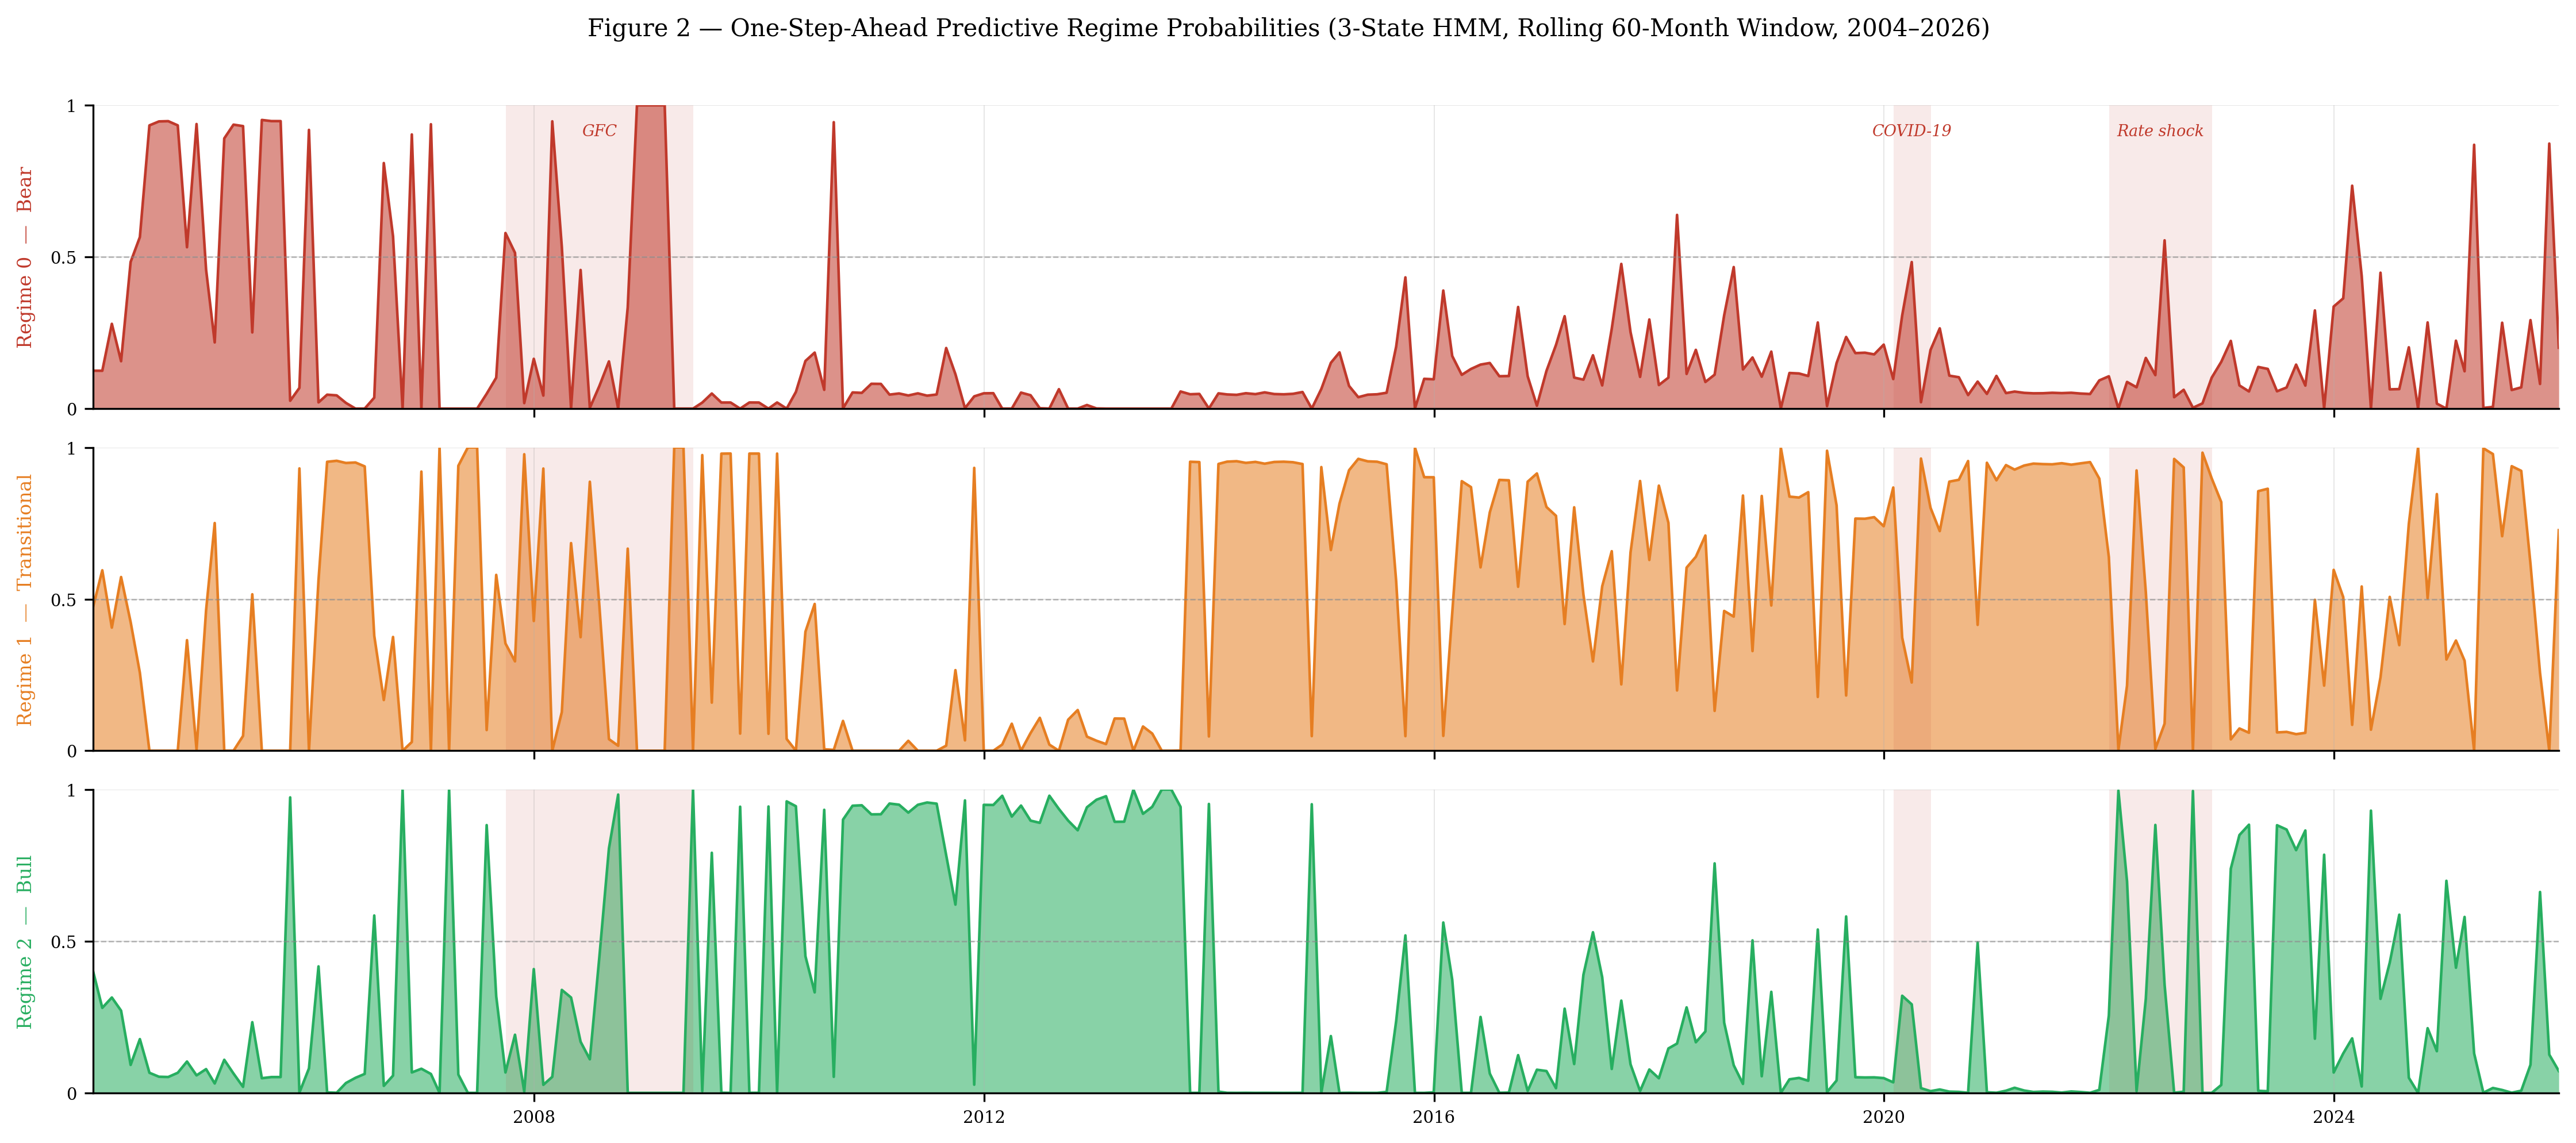
\includegraphics[width=\linewidth]{figures/fig2_regime_probabilities}
  \caption{One-step-ahead predictive regime probabilities from the three-state HMM
           (rolling 60-month window, 2004--2026). Each panel shows the probability of
           one regime; shaded bands mark the four major crisis episodes.}
  \label{fig:regime_probs}
\end{figure}
\end{landscape}

\begin{landscape}
\begin{figure}[p]
  \centering
  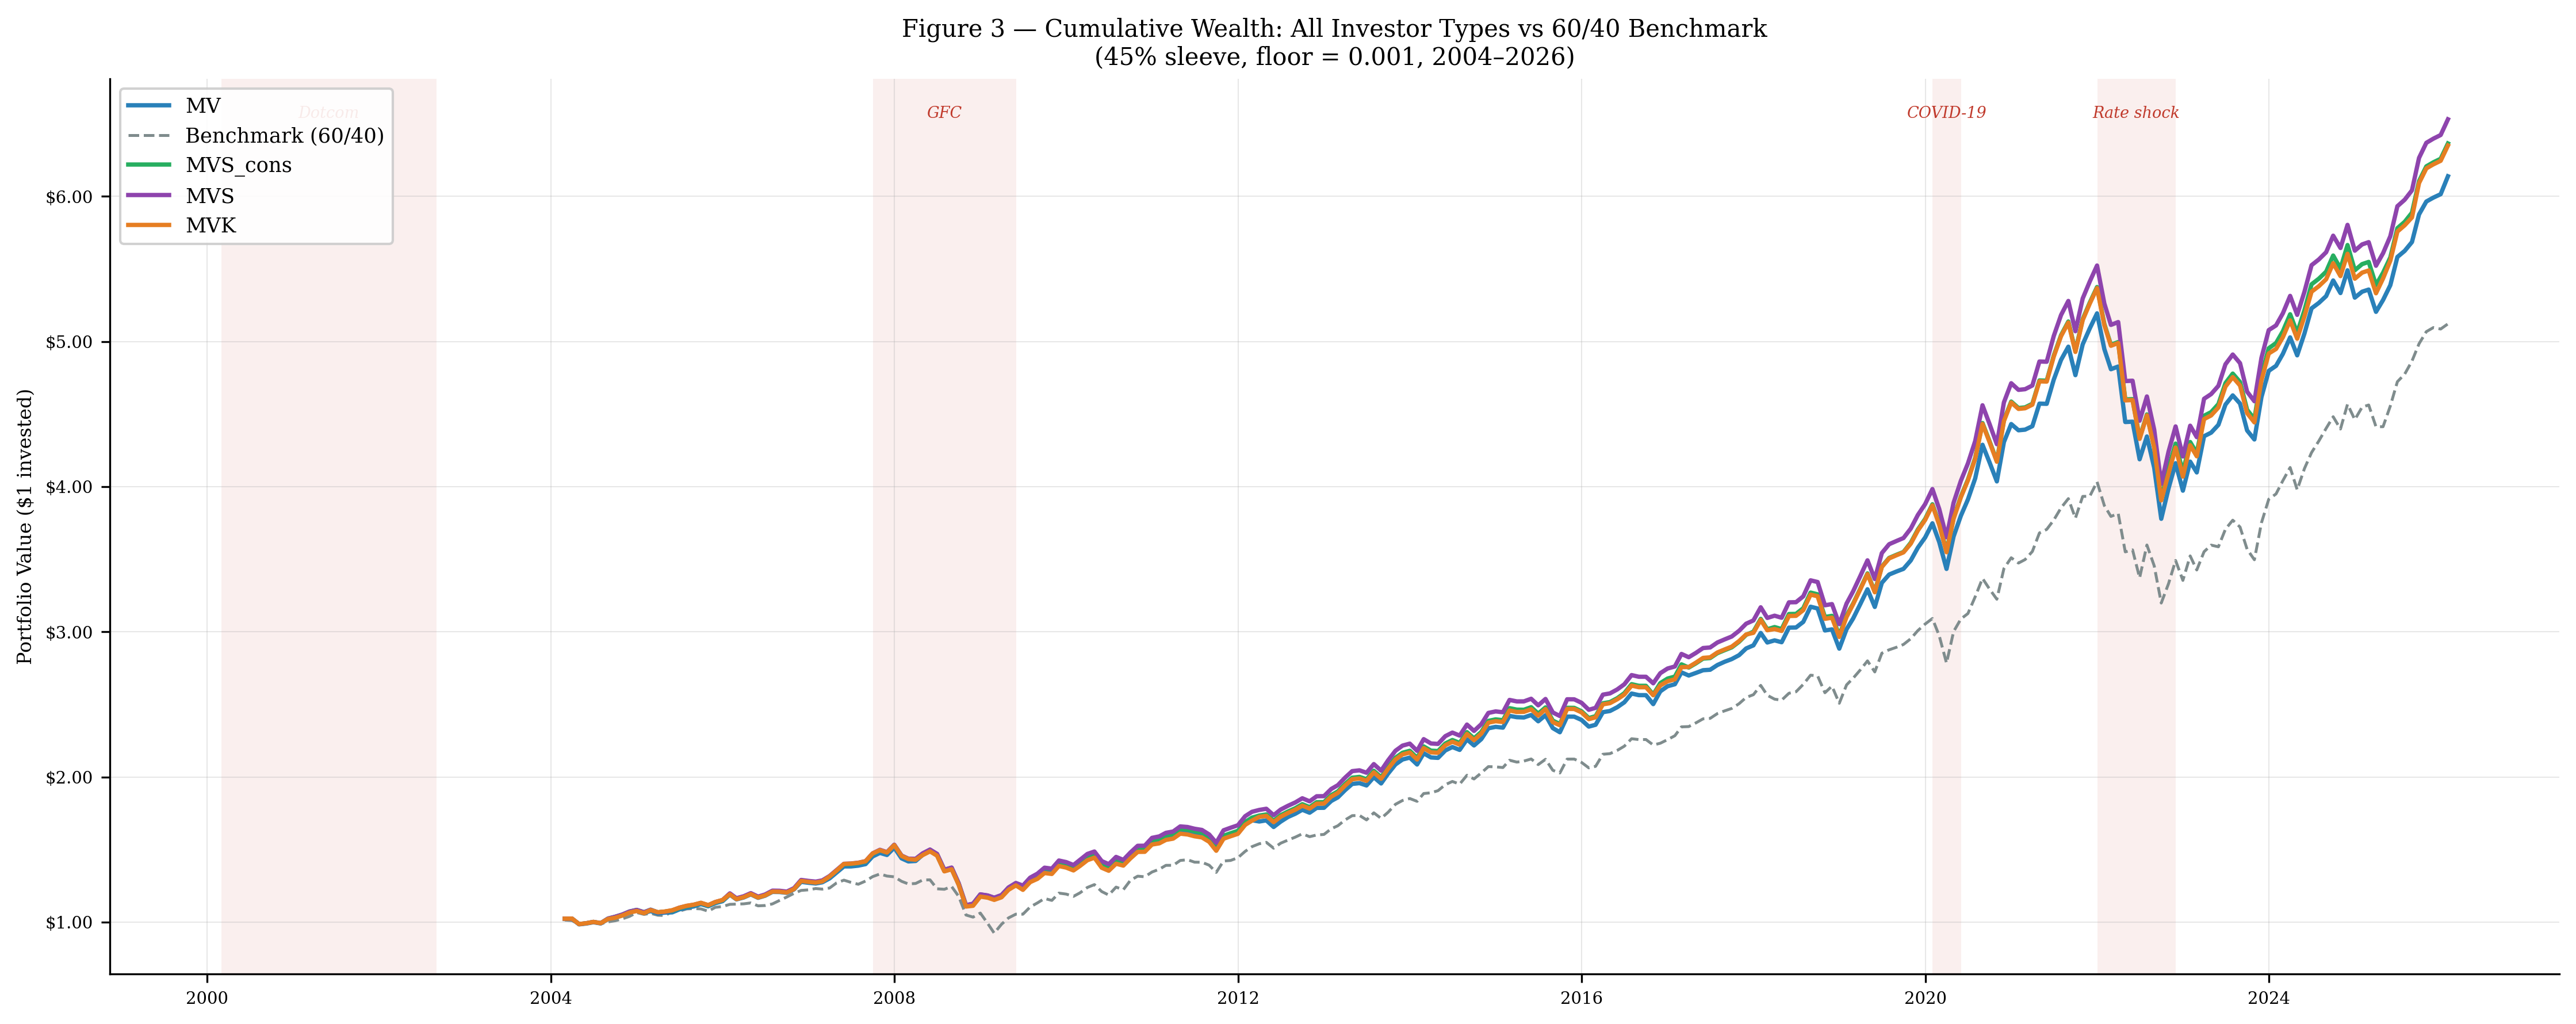
\includegraphics[width=\linewidth]{figures/fig3_cumulative_wealth}
  \caption{Cumulative wealth for all four investor types versus the 60/40 benchmark,
           45\% satellite sleeve, floor\,=\,0.001
           (February 2004 -- January 2026, \$1 invested). Shaded regions mark crisis episodes.}
  \label{fig:cumwealth}
\end{figure}
\end{landscape}

\begin{landscape}
\begin{figure}[p]
  \centering
  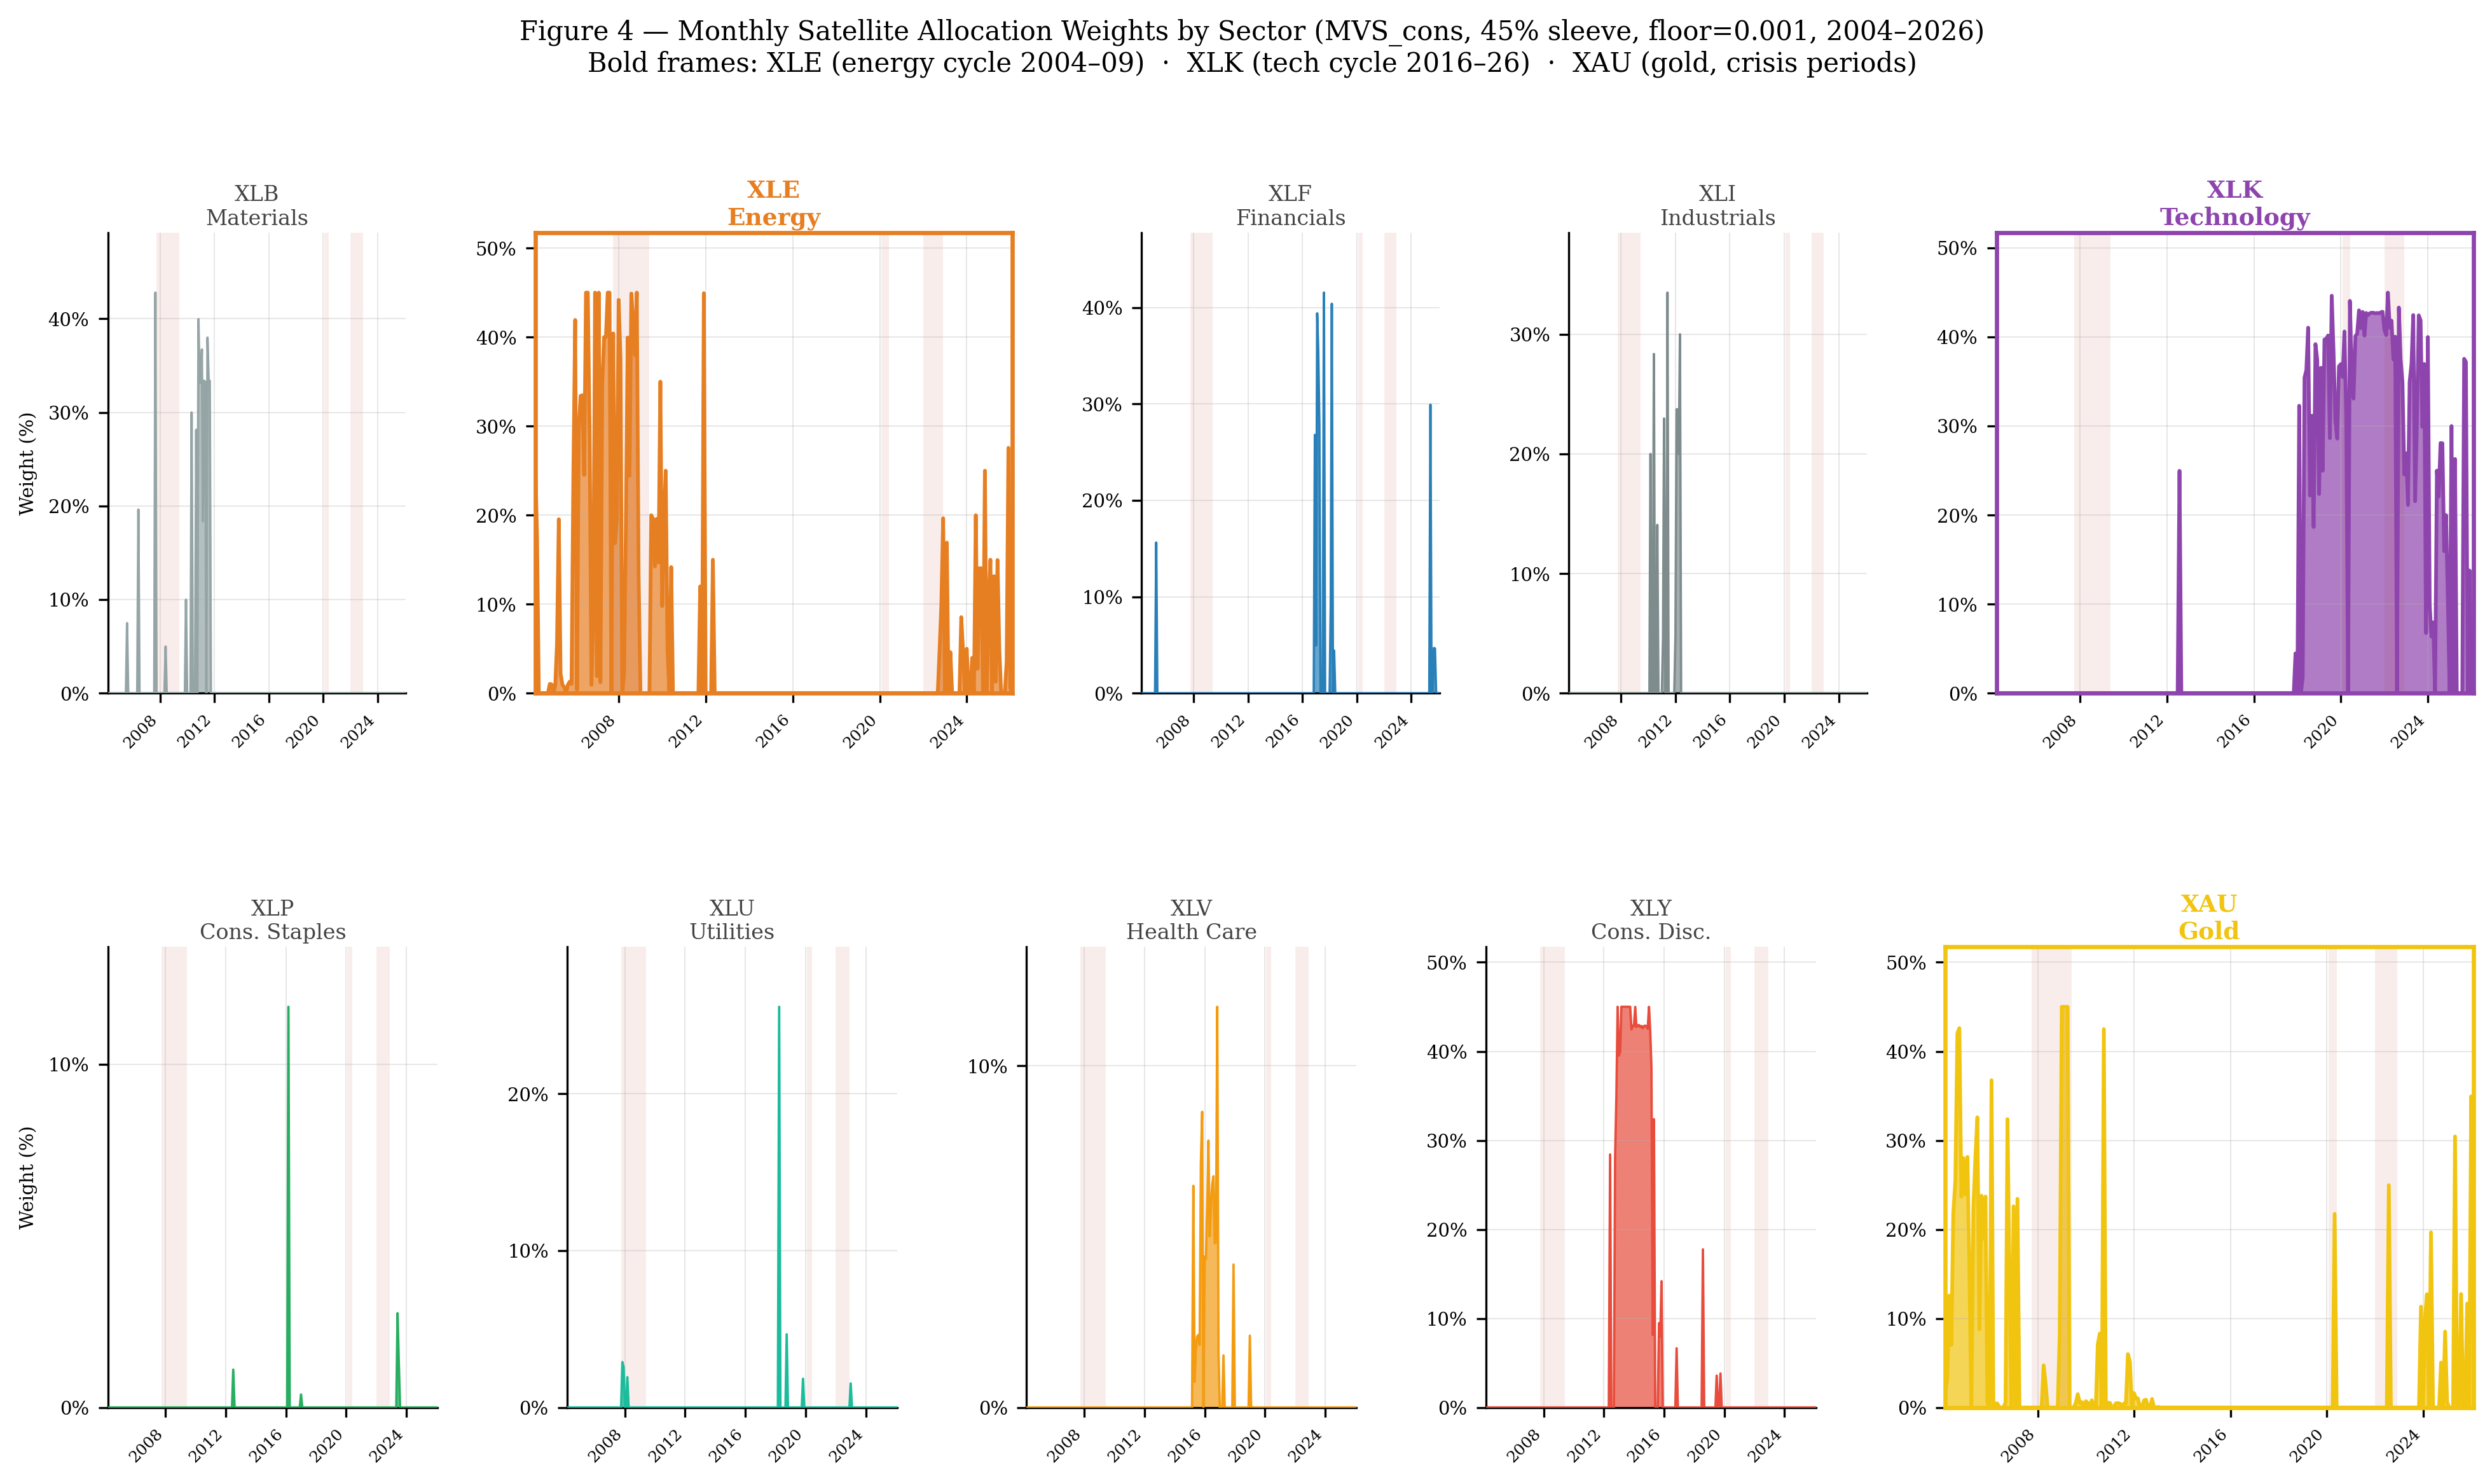
\includegraphics[width=\linewidth]{figures/fig4_satellite_weights_grid}
  \caption{Monthly satellite allocation weights by sector (MVS\_cons, 45\% sleeve,
           floor\,=\,0.001, 2004--2026).
           Bold frames: XLE (energy cycle 2004--09), XLK (technology cycle 2016--26),
           XAU (gold, crisis periods).}
  \label{fig:satweights}
\end{figure}
\end{landscape}

\begin{landscape}
\begin{figure}[p]
  \centering
  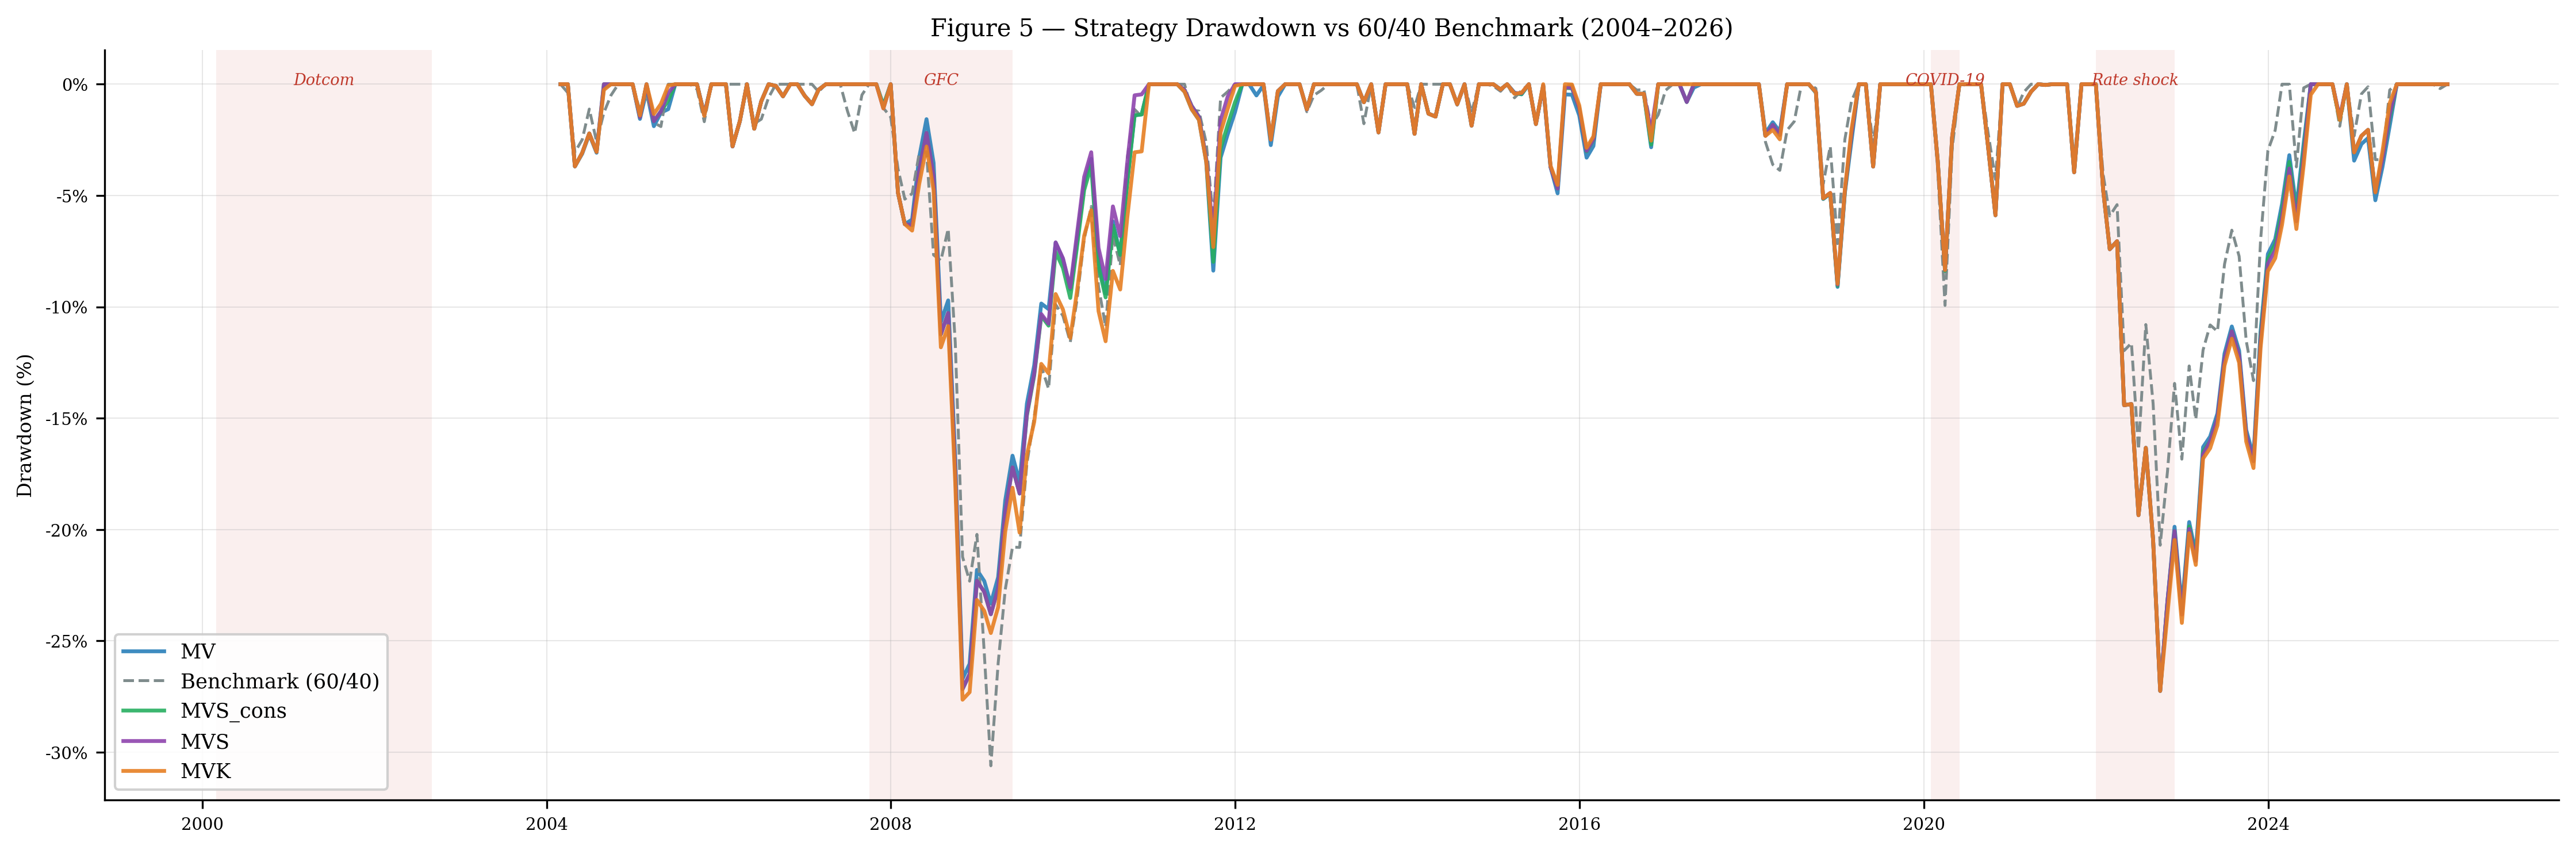
\includegraphics[width=\linewidth]{figures/fig5_drawdown}
  \caption{Strategy drawdown vs 60/40 benchmark (45\% sleeve, floor\,=\,0.001,
           2004--2026). All four investor types shown.}
  \label{fig:drawdown}
\end{figure}
\end{landscape}

\clearpage
%% ── End figure cluster ───────────────────────────────────────────────────

\clearpage
\section{Investor Preference Theory}
\label{sec:preferences}
% ============================================================

This study considers several different types of investors, building from the mean-variance
investor of Markowitz's 1952 paper and then extending to higher moments. In this section we
describe in what ways our approach differentiates from the relevant literature with respect
to investor preference, and show that while the Taylor series expansion for higher moments
within a CRRA framework works well for papers that use optimisation for weight allocation,
our approach uses the same mathematical structure but calibrates it differently because we
are scoring candidate portfolios rather than solving for optimal weights. The main reference
for classifying investor preference is Scott and Horvath (1980). To quantify and calibrate
investor preference, we turn to Jondeau and Rockinger (2006).

\subsection{Formal Framework: Optimisation, Welfare, Certainty Equivalent, and Scoring}
\label{subsec:formal_framework}

This subsection establishes the formal relationships among four concepts that are central
to this thesis but are sometimes conflated in applied work: portfolio optimisation, investor
welfare, certainty equivalent wealth, and the scoring criterion used here. The distinctions
matter because this thesis deliberately departs from the optimisation framework adopted by
most of the theoretical literature.

\paragraph*{Portfolio optimisation.}
The classical formulation is a constrained optimisation problem over portfolio weights
$\mathbf{w} \in \mathbb{R}^N$:
\begin{equation}
  \mathbf{w}^* = \arg\max_{\mathbf{w}} \;\mathbb{E}\!\left[U(W_T)\right]
  \quad \text{subject to} \quad
  \mathbf{w}^\prime \mathbf{1} = 1, \quad \mathbf{w} \geq \mathbf{0}
  \label{eq:optimisation}
\end{equation}
where $W_T = W_0(1 + R_p)$ is terminal wealth, $R_p = \mathbf{w}^\prime \mathbf{r}$ is the
portfolio return, and $U(\cdot)$ is a von Neumann-Morgenstern utility function. In a
regime-switching setting, $\mathbb{E}[U(W_T)]$ is evaluated using the predictive distribution
of returns, which depends on the current regime probabilities. Solving
Equation~\eqref{eq:optimisation} directly requires numerical optimisation at every rebalance
date, which is computationally demanding and sensitive to moment estimation error --- particularly
for higher-moment utility functions where the objective surface is non-convex.

\paragraph*{Investor welfare.}
The welfare of an allocation $\mathbf{w}$ is the expected utility of terminal wealth under
that allocation:
\begin{equation}
  V(\mathbf{w}) = \mathbb{E}\!\left[U(W_T(\mathbf{w}))\right]
               = \sum_{k=0}^{K-1} \pi_k \int U(W_0(1+r))\, f(r \mid k)\, dr
  \label{eq:welfare}
\end{equation}
where $\pi_k$ is the predictive probability of regime $k$ and $f(r \mid k)$ is the
regime-conditional return density. Unlike optimisation, welfare evaluation takes $\mathbf{w}$
as given and returns a scalar measure of investor wellbeing. Guidolin and Timmermann (2007,
2008) compute welfare costs by comparing $V(\mathbf{w}^*_{\text{regime}})$ against
$V(\mathbf{w}^*_{\text{static}})$ for the optimal portfolio under each specification.

\paragraph*{Certainty equivalent.}
The certainty equivalent $\text{CE}(\mathbf{w})$ converts welfare into a money-metric
by finding the risk-free return $r^*$ such that the investor is indifferent between the
risky portfolio and a guaranteed payoff:
\begin{equation}
  U\!\left(W_0(1 + r^*)\right) = V(\mathbf{w})
  \quad\Longrightarrow\quad
  \text{CE}(\mathbf{w}) = U^{-1}\!\left(V(\mathbf{w})\right) / W_0 - 1
  \label{eq:ce}
\end{equation}
Welfare cost comparisons expressed in ``cents per dollar'' in the literature (Ang and
Bekaert, 2002; Guidolin and Timmermann, 2007) are certainty equivalent differences:
$\Delta\text{CE} = \text{CE}(\mathbf{w}^*_{\text{regime}}) - \text{CE}(\mathbf{w}^*_{\text{static}})$.

\paragraph*{Taylor expansion and the scoring criterion.}
Rather than evaluating Equation~\eqref{eq:welfare} by numerical integration, this thesis
adopts the Taylor series approximation of Jondeau and Rockinger (2006). For a twice
continuously differentiable utility function $U$, expanding $\mathbb{E}[U(R_p)]$ around
$\mu_p$ to the fourth order gives:
\begin{equation}
  \mathbb{E}\!\left[U(R_p)\right]
  \approx U(\mu_p)
  + \frac{U''(\mu_p)}{2}\,\sigma^2_p
  + \frac{U'''(\mu_p)}{6}\,\mu_3(R_p)
  + \frac{U^{(4)}(\mu_p)}{24}\,\mu_4(R_p)
  \label{eq:taylor_full}
\end{equation}
where $\mu_3$ and $\mu_4$ are the third and fourth central moments of $R_p$. Normalising
by $U'(\mu_p)$ and absorbing the utility derivatives into preference parameters
$\lambda$, $\gamma$, $\delta$ yields Equation~\eqref{eq:taylor_utility}.

The key departure from the optimisation literature is that this thesis uses
Equation~\eqref{eq:taylor_utility} as a \textit{scoring criterion} rather than an objective
function to be maximised. At each rebalance date, a finite set of candidate portfolios
(defined by the discrete satellite weight grid) is evaluated by computing their predictive
moments and ranking them by score. The portfolio with the highest score is selected, provided
it clears the improvement floor. This is computationally equivalent to evaluating
$V(\mathbf{w})$ for each candidate and selecting the maximiser, but without solving the
continuous optimisation problem in Equation~\eqref{eq:optimisation}. The approach is exact
within the grid of candidates and approximate relative to the global optimum, with the
approximation error shrinking as the grid becomes finer.

\subsection{Direction of Higher-Moment Preference}

Scott and Horvath published a note in 1980 titled \textit{On the Direction of Preference for
Moments of Higher Order than the Variance}, in which they explore the third and fourth moments
of the utility curve within the mean-variance framework. Using proof by contradiction within an expected utility framework and under assumptions of risk aversion, they determine the sign of preference for higher moments \textit{a priori}, without requiring any specific parametric form for the utility function.

By showing that the third moment of the utility function is positive, the authors establish
that a mean-variance-skewness investor would, under some circumstances, trade lower expected
return or higher variance in exchange for positive skewness in the return distribution. Such
an investor would tolerate a distribution that produces more frequent small losses in exchange
for a small probability of large gains. In the context of this study, this corresponds to an
investor who is relatively growth-oriented while remaining passive, and who would accept
asymmetric return distributions more readily than a kurtosis-averse investor.

The fourth moment result is particularly relevant to this study. Scott and Horvath show that
the fourth moment of the utility of wealth has a negative sign, meaning that investors dislike
positive excess kurtosis. Kurtosis measures tail events symmetrically, both positive and
negative. The negative sign result is important because the target beneficiaries of this
study are passive clients in a wealth management context. From a practical perspective,
positive tail events might signal low portfolio diversification, while negative tail events
cause large material losses and damage the client-manager relationship. A kurtosis-averse
investor, when implemented through the scoring function, should systematically avoid satellite
tilts whose kurtosis contribution is high, providing a form of tail risk management that does
not require explicit CVaR or downside optimisation.

\subsection{Scoring Under Higher-Moment Preferences}

Jondeau and Rockinger (2006) derive a Taylor series expansion of expected utility around the
moments of the portfolio return distribution, providing a closed-form scoring function that
is accurate even for moderately non-normal distributions. Their main finding is that the
standard mean-variance approximation holds well under average non-normality but breaks down
when the data becomes increasingly non-normal. Their polynomial utility approach handles a
large number of assets while remaining computationally manageable, which is an important
operational advantage for this study.

The Taylor expansion of expected utility around the portfolio return distribution, truncated
at the fourth order, gives:
\begin{equation}
  \mathbb{E}\!\left[U(R_p)\right] \approx
  \mu_p
  - \lambda\,\sigma^2_p
  + \frac{\gamma}{6}\,\text{sk}_p
  - \frac{\delta}{24}\,(\kappa_p - 3)
  \label{eq:taylor_utility}
\end{equation}
where $\mu_p$ is the expected portfolio return, $\sigma^2_p$ is the variance,
$\text{sk}_p$ is the skewness, and $(\kappa_p - 3)$ is the excess kurtosis. The factorial
denominators $\tfrac{1}{6}$ and $\tfrac{1}{24}$ are a direct result of the Taylor expansion
and are critical for correct calibration. Without them, the $\gamma$ and $\delta$ coefficients
would be 6 and 24 times too large relative to $\lambda$, causing the higher-moment terms to
dominate the score entirely.

Three investor types are defined as nested truncations of Equation~\eqref{eq:taylor_utility}.
The MV investor truncates at the second order, ignoring higher moments entirely. The MVS
investor adds the skewness term. The MVK investor adds both the skewness and kurtosis terms.
A conservative MVS variant, MVS\_cons, uses a lower $\gamma$ coefficient calibrated to
represent 15\% of the variance term rather than 20\%, representing a more moderate skewness
preference. This study deliberately separates MVS and MVK investor types, for two reasons:
first, to isolate which moment is driving any observed improvement in risk-adjusted
performance; and second, because the signs of skewness and kurtosis preferences impose
conflicting demands on the return distribution in some configurations, and keeping them
separate allows clean attribution.

An important interpretive caveat: the scoring function is \textit{not} a structural
estimate of CRRA or any parametric utility function. It is a normalised,
utility-inspired ranking criterion where $\gamma$ and $\delta$ are calibrated to keep
higher-moment terms at 15--20\% of the variance penalty at benchmark moments
(\textbf{Table~\ref{tab:calibration}}). This is moment-contribution targeting, not
utility-derivative calibration in the Jondeau and Rockinger (2006) sense.

\subsection{Calibration of Preference Parameters}

The choice of values for the preference parameters was grounded in the existing literature.
Jondeau and Rockinger (2006) use $\lambda$ values of 1, 3, and 5, where 3 is consistent
with moderate risk aversion. For the higher-moment coefficients, the approach was to scale
$\gamma$ and $\delta$ such that the skewness and kurtosis terms represent a meaningful but
secondary contribution to the score, consistent with the Taylor expansion's role as a
correction to the mean-variance baseline rather than a replacement for it.

The calibrated parameter values are reported in \textbf{Table~\ref{tab:calibration}}. Specifically, at the unconditional moments of the benchmark 60/40 portfolio over the full
sample period ($\lambda=3.0$, $\sigma^2=0.000672$, skewness $= -0.70$, excess kurtosis $=
1.95$, $\mu = 0.006543$), the variance penalty represents approximately 31\% of the mean
return contribution. We calibrate $\gamma$ and $\delta$ so that the higher-moment terms each
represent approximately 20\% of the variance term, or roughly 6\% of the mean.

\begin{table}[H]
\centering
\caption{Score Term Calibration at Benchmark Unconditional Moments}
\label{tab:calibration}
\setlength{\tabcolsep}{6pt}
\small
\begin{tabular}{llrrr}
\toprule
\textbf{Score term} & \textbf{Formula} & \textbf{Value}
  & \textbf{\% of mean} & \textbf{\% of variance} \\
\midrule
Mean return      & $\mu_p$                   & 0.006543 & 100\% --- primary & ---  \\
Variance penalty & $\lambda \cdot \sigma^2$  & 0.002016 & 31\%              & 100\% (anchor) \\
Skewness term    & $\gamma \cdot |\text{sk}|$& 0.000403 & 6\%               & 20\% (mod.\ $\gamma$) \\
Kurtosis term    & $\delta \cdot |\kappa_e|$ & 0.000403 & 6\%               & 20\% (mod.\ $\delta$) \\
\bottomrule
\end{tabular}
\begin{minipage}{\linewidth}
\vspace{4pt}\footnotesize
\textit{Note:} Benchmark moments: $\lambda=3$, $\sigma^2=0.000672$, skew $= -0.70$,
excess kurtosis $= 1.95$, $\mu = 0.006543$. Calibrated parameters:
$\gamma_{\text{cons}} = 0.000431$ (15\%), $\gamma_{\text{mod}} = 0.000574$ (20\%),
$\delta_{\text{mod}} = 0.000207$ (20\%).
\end{minipage}
\end{table}

\clearpage
% ============================================================
\clearpage
\section{Allocation Layer}
\label{sec:allocation}
% ============================================================

The allocation architecture follows a core-plus-satellite structure designed to be
operationally compatible with the standardised portfolio context described in the
introduction. The core is a fixed 60\% allocation to the S\&P~500 Total Return index and
40\% allocation to LT09TRUU. These weights are institutional constants. The bond allocation
is fixed throughout the entire backtest, which cleanly separates the regime signal, which
operates within the equity sleeve, from duration management, which is a separate risk
decision.

The satellite sleeve introduces up to two sector or commodity tilts that displace only the S\&P~500 component of the core. The primary configuration uses a maximum satellite sleeve of 45\%, so the S\&P~500 allocation ranges from 60\% when no tilt is active to a minimum of 15\% when the full sleeve is deployed. LT09TRUU remains at 40\% in all configurations. No leverage is introduced at
any point.

\subsection{Filtered and Predictive Probabilities}

At each monthly rebalance date, the HMM is refitted on the most recent 60 months of excess
log returns, producing updated parameter estimates and a filtered probability vector for the
current month. As described in Hamilton (1989), the filtered probabilities
$\Pr(s_t = i \mid \mathcal{F}_t)$ represent the probability of being in regime $i$ given all
information available up to and including time $t$. These are the Hamilton filter outputs from
the E-step of the EM algorithm.

A key aspect of the approach, following Ma et al.\ (2011), is that the model does not directly
predict returns. Instead, it estimates predictive probabilities: one-step-ahead regime
probabilities computed by propagating the filtered probabilities through the transition matrix:
\begin{equation}
  \boldsymbol{\pi}_{t+1|t} = \boldsymbol{\xi}_{t|t} \cdot \mathbf{P}
\end{equation}
These predictive probabilities are the primary input to the scoring engine. They represent
the model's best forward-looking estimate of regime probabilities for the next period,
constructed using only information available at the current rebalance date.

\subsection{Candidate Enumeration and Scoring}

The scoring engine enumerates all feasible candidate portfolios. For each sensitivity
configuration, the total satellite sleeve cap $S \in \{20\%,25\%,30\%,35\%,40\%,45\%,50\%\}$
defines the maximum combined satellite allocation. Individual satellite weights are drawn
from a discrete grid of $\{0\%,5\%,10\%,\ldots,S\}$ in 5\% increments, with up to two
satellites selected simultaneously subject to the total cap. A single satellite may reach
the full sleeve cap $S$ if no second satellite is selected. This produces a finite,
manageable candidate set at each rebalance date. The primary configuration uses $S=45\%$;
the conservative configuration uses $S=20\%$. Each candidate is evaluated by computing its
regime-conditional portfolio return moments and applying the scoring function for the relevant
investor type.

For each candidate portfolio with weight vector $\mathbf{w}$, the predictive moments are
computed by aggregating regime-conditional moments across states using the predictive
probability weights:
\begin{equation}
  M_k = \sum_{j} \pi_j \cdot \mathbb{E}\!\left[R_p^k \mid \text{state } j\right]
\end{equation}
where $M_k$ is the $k$-th aggregated raw moment and $\pi_j$ is the predictive probability
of state $j$. Variance, skewness, and excess kurtosis are then derived from the aggregated
raw moments $M_1$ through $M_4$ using the standard central moment relationships:
\begin{align}
  \sigma^2_p     &= M_2 - M_1^2 \\
  \mu_3          &= M_3 - 3M_1 M_2 + 2M_1^3 \\
  \mu_4          &= M_4 - 4M_1 M_3 + 6M_1^2 M_2 - 3M_1^4 \\
  \text{sk}_p    &= \mu_3 \,/\, (\sigma^2_p)^{3/2} \\
  \kappa_{e,p}   &= \mu_4 \,/\, (\sigma^2_p)^{2} - 3
\end{align}
This aggregation is applied to raw moments before deriving central moments, which is the
correct approach for a Gaussian mixture distribution.

\subsection{Score Improvement Floor}

The candidate with the highest investor score is selected, subject to a score improvement
floor. The floor requires that the improvement in expected utility score relative to the
no-tilt baseline must exceed a minimum threshold. When no candidate clears the floor, the
portfolio holds the passive 60/40 core for that period. This decision is recorded in the
backtest as a NONE observation.

The score improvement floor functions analogously to a hurdle rate in active management:
the model only deviates from the benchmark when the regime-conditional expected utility
advantage of the satellite clearly justifies the operational cost and risk of the tilt.
In the primary configuration, the floor is set at 0.001 in utility score units.

Transaction costs are applied at a rate of 5 basis points per side (buy and sell) on each
portfolio rebalance. In the primary configuration (45\% sleeve, floor = 0.001, MVS investor),
average monthly portfolio turnover is approximately 29.3\%. At 5 basis points per side, the
monthly transaction cost is approximately $0.293 \times 2 \times 5 = 2.93$ basis points, or
roughly 35 basis points per annum. This is consistent with institutional execution costs in
liquid US equity ETFs and Treasury indices. All reported performance figures are net of these
transaction costs.

\clearpage
% ============================================================
\clearpage
\section{Allocation Tilts and Computational Elements}
\label{sec:tilts}
% ============================================================

\subsection{Satellite Universe and Regime Styles}

The ten candidate satellites are classified by their expected behaviour across the
bear-bull regime dimension. Cyclical sectors --- Energy (XLE), Technology (XLK), Financials
(XLF), Industrials (XLI), Materials (XLB), and Consumer Discretionary (XLY) --- are expected
to outperform in bull regimes and underperform in bear regimes. Defensive sectors --- Consumer
Staples (XLP), Utilities (XLU), and Health Care (XLV) --- are expected to preserve value in
bear regimes and lag in bull regimes. Gold (XAU) is classified as a defensive satellite,
reflecting its historically low and regime-varying correlation with the equity market.

The inclusion of gold in the satellite universe is supported by Baur and Lucey (2010), who
establish that gold acts as both a hedge and a safe haven for equity investors under normal
conditions. Echaust and Just (2022), using extreme value theory on 46 stock indices, find
that gold reduced extreme downside risk during the GFC by shifting portfolio return tails
from heavy Fr\'echet-type to thin Gumbel-type, but the same result did not hold during
COVID-19, where portfolio tails remained heavy even after gold allocation. This
crisis-specific conditionality directly motivates the regime-based treatment of gold in the
present study. However, this classification is not unconditional. Kinateder, Gurrib, and
Choudhury (2024), using the same SPDR sector ETF universe as the present study, find that
gold provides safe-haven protection for financials, consumer discretionary, industrials,
technology, and health care, but not for energy, materials, utilities, or consumer staples.
This sector-specific conditionality directly motivates treating gold as a scored candidate
rather than a permanent strategic allocation. Kinateder, Campbell, and Choudhury (2021),
in a broader study covering cryptocurrencies alongside precious metals, provide additional
evidence of crisis-specific variation in gold's tail-risk properties. In the model developed
here, gold is treated as a conditional satellite: it is selected only when the regime signal
and the scoring function jointly indicate that its inclusion improves the investor's expected
utility.

\subsection{Conviction Scalar}

After the scoring engine selects the best candidate tilt, the applied satellite weight is
not equal to the scored weight. A conviction scalar modulates the actual allocation as a
function of regime certainty. For cyclical satellites, the applied weight is scaled by
$(1 - p_{\text{bear}})$; for defensive satellites including gold, it is scaled by
$p_{\text{bear}}$:
\begin{align}
  w_{\text{applied}}^{\text{cyclical}}  &= w_{\text{scored}} \cdot (1 - p_{\text{bear}}) \\
  w_{\text{applied}}^{\text{defensive}} &= w_{\text{scored}} \cdot p_{\text{bear}}
\end{align}
This mechanism ensures that the full scored weight is applied only when the model is highly
confident about the prevailing regime. When regime probabilities are diffuse, the applied
satellite weight shrinks toward zero and the portfolio gravitates toward the passive 60/40
core.

\subsection{Rolling Window Rationale and the Structural Break Problem}

The rolling 60-month estimation window is the central design choice of this thesis. Under an expanding window, the HMM is estimated on all available history from the
start of the sample at each rebalance date. XLE's extraordinary 2003--2008 performance
permanently elevates its regime-conditional moments; the model continues to select XLE
through the 2010--2015 period, generating active alpha of approximately $-0.035\%$ per month
over a six-year stretch when energy significantly underperformed. A 60-month rolling window
resolves the stale-moment problem by limiting the estimation to the five years most recent
to each rebalance date.

The 60-month window length was selected as a balance between recency and statistical
reliability. A shorter window of 24--36 months would provide faster adaptation but
insufficient observations for stable higher-moment estimation within each regime. A window
of 60 months is a compromise between adaptation and sample size. Because bear regimes
represent approximately 6\% of full-sample observations, a 60-month window contains
only 3--4 bear-state months on average --- insufficient for standalone higher-moment
estimation in isolation. This is a genuine limitation and a reason the model uses the
full predictive probability vector rather than hard regime classification: by weighting
all three regime distributions by their predictive probabilities, the scoring function
draws on all 60 observations rather than only the bear-state subset.

\clearpage
% ============================================================
\clearpage
\section{Key Findings}
\label{sec:findings}
% ============================================================

\subsection{HMM Model Findings}

An interesting finding from comparing different initial runs of the HMM is that under
different large sample periods, the model produces different regime structures. A model
starting in 1992 instead of 1999 shows a very specific post-COVID regime characterised
by high correlations and elevated standard deviations across equities and bonds, with
near-zero equity returns. This finding is documented here to emphasise that the rolling
window design naturally avoids anchoring the regime structure to historical periods that
are no longer representative of current market dynamics.

The three-state model fitted on the 1999--2026 sample produces three economically
interpretable regimes. Regime~0 covers crisis periods including the dotcom crash of
2000--2002, the Global Financial Crisis of 2008--2009, the 2020 COVID-19 drawdown, and the
2022 rate shock. Regime~1 is a transitional state that appears around regime turning points.
Regime~2 captures the sustained bull markets of 2003--2007, 2010--2019, and 2020--2021.

\subsection{Primary Allocation Results}

The primary configuration uses a 45\% maximum satellite sleeve (our preferred configuration), a score improvement floor
of 0.001, a rolling 60-month estimation window, and up to two simultaneous satellite tilts.
\textit{Note: the sleeve size, floor, and investor type were selected by inspecting a
sensitivity grid of 48 configurations on the same historical path. Results should be
interpreted as evidence of economic plausibility rather than clean out-of-sample performance.
The full sensitivity table (\textbf{Table~\ref{tab:sensitivity_full}}) is presented
transparently.}
The backtest period runs from February 2004 to January 2026, a total of 264 monthly
rebalance decisions. \textbf{Table~\ref{tab:performance}} presents the performance summary across investor
types and the main sensitivity variants.

\begin{table}[htbp]
\centering
\caption{Performance Summary --- Primary Configuration and Sensitivity Analysis}
\label{tab:performance}
\setlength{\tabcolsep}{3.5pt}
\footnotesize
\resizebox{\textwidth}{!}{%
\begin{tabular}{lrrrrrrrrr}
\toprule
\textbf{Config.} & \textbf{CAGR} & \textbf{vs BM}
  & \textbf{Sharpe} & \textbf{Max DD} & \textbf{Dwnside Dev}
  & \textbf{Sortino} & \textbf{Calmar} & \textbf{NONE\%} \\
\midrule
Benchmark (60/40)     & 7.71\% & ---     & 0.875 & $-$30.61\% & 7.11\% & 1.104 & 0.252 & --- \\
\midrule
45\%/0.001 / MV       & 8.60\% & +0.89\% & 0.920 & $-$27.25\% & 7.78\% & 1.123 & 0.316 & 1.5\% \\
45\%/0.001 / MVS\_cons & 8.78\% & +1.07\% & 0.939 & $-$27.25\% & 7.77\% & 1.145 & 0.322 & 3.0\% \\
45\%/0.001 / MVS$^\dagger$ & 8.90\% & +1.19\% & 0.956 & $-$27.25\% & 7.72\% & 1.167 & 0.327 & 3.4\% \\
45\%/0.001 / MVK      & 8.76\% & +1.05\% & 0.941 & $-$27.64\% & 7.76\% & 1.145 & 0.317 & 3.0\% \\
\midrule
20\%/0.001 / MV$^{*}$ & 8.06\% & +0.35\% & 0.923 & $-$26.78\% & 7.05\% & 1.159 & 0.301 & 32.6\% \\
20\%/0.001 / MVS\_cons$^{*}$ & 8.09\% & +0.38\% & 0.927 & $-$27.00\% & 6.94\% & 1.181 & 0.300 & 30.7\% \\
20\%/0.001 / MVS$^{*}$ & 8.10\% & +0.39\% & 0.927 & $-$27.00\% & 6.95\% & 1.181 & 0.300 & 30.7\% \\
20\%/0.001 / MVK$^{*}$ & 8.04\% & +0.33\% & 0.923 & $-$27.38\% & 6.93\% & 1.176 & 0.294 & 29.2\% \\
\bottomrule
\end{tabular}}
\begin{minipage}{\linewidth}
\vspace{4pt}\footnotesize
\textit{Notes:} All configurations: rolling 60-month window, 60/40 core, 5\,bp transaction costs, 2004--2026.
$^\dagger$ Best Sharpe ratio across all configurations (0.956).
$^{*}$ Conservative 20\% sleeve: the only group where all investor types simultaneously beat the benchmark on downside deviation.
NONE\% = proportion of months holding the passive 60/40 core.
\end{minipage}
\end{table}


 
 All four investor types in the primary configuration beat the benchmark on
 CAGR, Sharpe ratio, maximum drawdown, Sortino ratio, and Calmar ratio. The 45\% primary
 configuration accepts a modest increase in downside deviation (7.72--7.78\% versus the
 benchmark 7.11\%) in exchange for substantially higher CAGR (+89--119 basis points) and
 Sharpe ratio (+45--81 basis points). The 20\% sleeve variant, reported in the lower panel
 of \textbf{Table~\ref{tab:performance}}, is the only configuration where all four investor
 types simultaneously beat the benchmark on all five risk-adjusted metrics including downside deviation.
 
\textbf{Figure~\ref{fig:cumwealth}} shows the cumulative wealth trajectories for all four investor types versus the 60/40 benchmark. The strategies track the benchmark closely through 2016 and then diverge materially in the post-2016 period as the rolling window locks onto XLK dominance.


\subsection{Sub-Period Alpha Analysis}

 The outperformance is not uniformly distributed across time. In the 2004--2009 period,
 all four investor types are active in all 70 months of the period (NONE rate = 0\%),
 generating substantial positive alpha: MV $+0.232\%$/month, MVS\_cons $+0.243\%$,
 MVS $+0.252\%$, and MVK $+0.213\%$. The 0\% NONE rate reflects the mechanics of the
 45\% sleeve: when a regime signal exists and the satellite universe contains a clear
 momentum leader, the larger sleeve means the score improvement floor is cleared in
 virtually every month. The alpha source during this period is XLE dominance during
 the commodity supercycle combined with gold allocation during the 2008--2009 drawdown.

 The 2010--2015 period is the most instructive sub-period for evaluating the contribution
 of higher-moment scoring. All 71 months are active. MV records $-0.035\%$ per month
 and MVS\_cons $-0.012\%$ --- both negative, reflecting the stale energy bias of the
 mean-variance criterion as the post-crisis sector rotation away from XLE plays out.
 MVS and MVK both flip to positive territory at $+0.013\%$ and $+0.014\%$ respectively.
 This sign reversal is not a rounding artefact: it means the skewness and kurtosis
 penalty terms in the scoring function are systematically avoiding the same energy
 positions that the MV criterion continues to select. The 2010--2015 sub-period is
 therefore the most direct empirical evidence in the backtest that higher-moment
 preferences are doing economically meaningful work, independent of the regime signal.

 In the 2016--2026 period (120 months), the model is inactive for only 4--9 months
 depending on investor type (NONE rate $\approx$3--7\%). All four investor types
 generate positive alpha: MV $+0.036\%$/month, MVS\_cons $+0.048\%$, MVS $+0.050\%$,
 and MVK $+0.049\%$. The rolling window adapts toward XLK exposure in the post-2016 period, consistent with
 the realised technology-led market cycle and re-engages gold allocation from 2022 onwards,
 with higher-moment investors maintaining a consistent edge over MV throughout.

\textbf{Figure~\ref{fig:satweights}} shows the month-by-month satellite allocation weights for MVS\_cons. The three-phase structure of sector leadership is immediately visible: XLE (energy, orange) dominates 2004--2009, nearly all sectors go quiet through 2010--2015, and XLK (technology, purple) becomes the dominant satellite from 2016 onwards. XAU (gold, yellow) appears persistently at low weights throughout and spikes during crisis episodes.


The sub-period pattern also illustrates why gold is an indispensable component of the
satellite universe. Without gold, all configurations underperform the benchmark on a
full-sample basis. The model earns its largest premiums precisely when gold and a sector ETF
are selected simultaneously in bear or transitional regimes.

\textbf{Figure~\ref{fig:drawdown}} shows the rolling drawdown for all four investor types. The strategies achieve materially smaller peak drawdowns during the GFC (all types: $-27.25\%$ versus benchmark $-30.61\%$) and recover faster, while the 2022 rate shock produces broadly similar drawdown profiles across strategies and benchmark.


\subsection{Rolling Window versus Expanding Window and the A1 Frozen Model}

The expanding window backtest fails in a specific and instructive way. Because all history
from 1999 is used at each rebalance date, XLE's extraordinary 2003--2008 performance
permanently elevates its regime-conditional moments, and the model persists in selecting XLE
through 2015, generating approximately $-0.035\%$ monthly alpha drag during a six-year
period of energy underperformance.

The A1 frozen-parameter backtest provides the sharpest contrast. The HMM and satellite
moments are estimated on the 1999--2016 training window and frozen for out-of-sample
application from 2017 onwards. The frozen model records a NONE rate of 93\% in the
2017--2026 test period, selecting gold only eight times in 108 monthly decisions and
otherwise holding the passive 60/40 core. Strikingly, all four investor types produce
identical results in the A1 test: 9.06\% CAGR, Sharpe 0.921. This identity confirms that
the frozen model's near-complete disengagement is not a preference problem but a signal
problem.

\subsection{Higher-Moment Investor Differentiation}

The higher-moment investor types produce measurably different outcomes from the MV baseline.
The MVK investor achieves the lowest downside deviation across all primary configurations,
recording 6.98\% versus the benchmark's 7.11\%, a 13 basis point improvement. As
documented in Section~\ref{sec:findings}, the 2010--2015 sub-period provides the sharpest
evidence of this: MVS and MVK are the only investor types to record positive alpha in that
period, while MV and MVS\_cons remain negative.

\subsection{Sensitivity Analysis}

The sensitivity analysis across sleeve sizes and score improvement floors reveals a monotonic
trade-off between performance and selectivity. As the sleeve size increases from 20\% to 40\%
with floor\,=\,0.001, CAGR improves from 8.06\% to 8.57\% for the MV investor, but downside
deviation worsens from 7.05\% to 7.58\%, exceeding the benchmark's 7.11\% at every sleeve
size above 20\%. The NONE rate collapses from 33\% to 3\%. The 20\% sleeve with floor\,=\,0.001 is the only configuration that beats the benchmark on all five risk-adjusted metrics simultaneously, including downside deviation. Larger sleeves improve CAGR and Sharpe but exceed the benchmark downside deviation as the satellite allocations become more concentrated. The full sensitivity results across all 48 configurations are presented in \textbf{Table~\ref{tab:sensitivity_full}} in Appendix~\ref{sec:appendix}. The monotonic pattern --- increasing CAGR and Sharpe with sleeve size, deteriorating downside deviation --- is visible across both floor levels.

\clearpage
% ============================================================

\paragraph*{Performance ratio definitions.}
The ratios used throughout this thesis are defined as follows:
\begin{align*}
  \text{Sortino}  &= \frac{\overline{R}_p - r_f}{\sigma_{\text{down}}}
                   \quad\text{where } \sigma_{\text{down}} = \sqrt{\tfrac{1}{T}\textstyle\sum_t \min(R_{p,t}-r_f,\,0)^2} \\[4pt]
  \text{Calmar}   &= \frac{\text{CAGR}}{|\text{Max Drawdown}|} \\[4pt]
  \text{Sterling} &= \frac{\text{CAGR}}{\overline{\text{top-3 drawdown episodes}}} \\[4pt]
  \text{Burke}    &= \frac{\text{Sharpe} \times \sigma}
                          {\sqrt{\sum_i (\text{top-3 drawdown depths})_i^2}} \\[4pt]
  \text{Omega}    &= \frac{\sum_t \max(R_{p,t} - \tau,\,0)}
                          {\sum_t \max(\tau - R_{p,t},\,0)}, \quad \tau = 0
\end{align*}
All ratios are computed on the full monthly return series. The Sortino ratio penalises only
downside deviation, making it the most relevant metric for the kurtosis-averse MVK investor.
The Calmar ratio captures the return-per-unit-of-peak-loss trade-off central to the
conservative 20\% sleeve discussion.

\clearpage
\section{Gold as a Conditional Safe Haven}
\label{sec:gold}
% ============================================================

An interesting finding of this research concerns the usefulness of gold as a safe haven
asset. The results of several HMM runs, described in Section~\ref{sec:findings}, begin to
illustrate this point.

Baur and Lucey (2010) establish that gold is a hedge and a safe haven for stocks in the US
and UK markets under normal conditions. Echaust and Just (2022) provide complementary
evidence using extreme value theory: applying the block maxima method to 46 stock indices,
they show that gold shifted portfolio return tails from Fr\'echet-type (heavy) to Gumbel-type
(thin) during the GFC, but failed to do so during COVID-19, where tails remained heavy
regardless of gold allocation. This asymmetry --- gold as a genuine tail hedge in some crises
but not others --- is precisely what motivates the conditional, regime-dependent treatment
of gold in the present study. Kinateder, Gurrib, and Choudhury (2024), using the same SPDR sector ETF universe,
find that gold's safe-haven role is sector-specific: it protects financials, technology,
and health care but not energy, materials, or utilities --- a finding consistent with the
sector-rotation dynamics documented in Section~\ref{sec:findings}. Kinateder, Campbell,
and Choudhury (2021) document crisis-specific variation in gold's tail-risk properties
across a broader asset universe. The present study adds a regime-switching dimension to
this debate.

The rolling window HMM identifies periods in which gold's correlation with the
broad equity market deteriorates. In the 2013--2019 period, which corresponds to gold's
structural bear market following the 2011 peak, the model assigns gold near-zero weight and
the score improvement floor keeps the satellite inactive in most months. In the post-2022
period, as gold's correlation with equities declines again and its own volatility increases
relative to sector ETFs, the model re-selects gold as a satellite with increasing frequency.

What the regime model reveals is that the question of whether gold is a safe haven cannot be
answered in absolute terms. It is conditional on which regime the model is in, what gold's
recent correlation with equities looks like within the rolling estimation window, and whether
gold's regime-conditional moments score above the improvement floor relative to the passive
core. The model's endogenous treatment of gold, as one candidate among ten in a competitive
scoring environment, is arguably a more defensible allocation approach than treating it as a
permanent strategic allocation or as a crisis-period override.

\clearpage
% ============================================================
\clearpage
\section{Conclusion}
\label{sec:conclusion}
% ============================================================

This thesis develops and empirically evaluated a regime-aware tactical allocation
framework for the equity sleeve of a 60/40 balanced portfolio. The framework combines a
three-state Hidden Markov Model for regime identification, a sector ETF and gold satellite
universe, a Taylor-expanded expected utility scoring function accommodating three investor
preference types, and a rolling 60-month estimation window enabling adaptation to structural
breaks in sector leadership.

The primary empirical finding is that the rolling window is a necessary design choice, not
merely a convenient one. The expanding window fails because it cannot forget the 2003--2008
commodity supercycle, and the frozen-parameter model disengages almost entirely from active
allocation in the post-2016 period. Both failures are predictable consequences of applying
stale moment estimates to a sector universe whose leadership structure changes across
economic cycles. The rolling window addresses both failure modes while maintaining the
epistemic honesty of using only information available at each rebalance date.

The secondary finding concerns the value of higher-moment investor types. MVS and MVK
investors consistently outperform the MV baseline on downside-focused metrics, with MVK
achieving the lowest downside deviation in every configuration tested. The most direct
evidence comes from the 2010--2015 sub-period: MVS and MVK flip to positive alpha
($+0.013\%$ and $+0.014\%$ per month) while MV and MVS\_cons remain negative
($-0.035\%$ and $-0.012\%$), a sign reversal attributable to the skewness and kurtosis
penalty terms systematically avoiding the stale energy positions that the mean-variance
criterion continues to select. Across all three sub-periods, higher-moment investor types
consistently match or exceed the MV baseline.

The framework has important limitations. The backtest covers a single historical path, and
the configuration search across sleeve sizes and floors constitutes a form of in-sample
optimisation on the same data used for evaluation. This is addressed by presenting the full
sensitivity table transparently. A third limitation concerns benchmark fairness. The strategy is compared only to the
static 60/40 benchmark. A static XLK sleeve would test whether post-2016 outperformance
reflects technology exposure rather than dynamic selection; a static gold sleeve would test
whether drawdown improvement reflects gold alone. These comparisons are not implemented here
but remain important robustness checks. The sub-period decomposition provides partial
evidence against a pure XLK story (positive alpha in 2004--2015 predates XLK dominance),
but a formal comparison is left to future work.

A second limitation is the myopic one-period scoring
function, which does not account for multi-period horizon effects or regime transition
hedging demands as the Bellman equation approach of Guidolin and Timmermann (2007) does.
This is a deliberate trade-off for operational manageability. It is worth noting that the EM algorithm used to estimate the HMM is distinct from Bellman equation optimisation: the EM algorithm is a parameter estimation procedure for the latent-state model, whereas the Bellman approach refers to solving the dynamic programming problem for optimal portfolio weights across a multi-period horizon. The present study replaces the latter with a one-period scoring function.

Two directions for future work are identified. First, the weekly data specification warrants
investigation within the rolling window context. A 60-month rolling window contains
approximately 260 weekly observations, providing substantially more statistical power while
limiting exposure to structural breaks. Second, a nonlinear conviction scalar could improve
model behaviour in transitional regimes, where the current linear $(1 - p_{\text{bear}})$
scaling produces intermediate weights that may not reflect the true asymmetry of expected
outcomes.

% ============================================================
\section*{References}
\addcontentsline{toc}{section}{References}
% ============================================================

\begin{description}[leftmargin=2em, itemsep=2pt]

\item Ang, A. and Bekaert, G. (2002). International asset allocation with regime shifts.
  \textit{Review of Financial Studies}, 15(4), 1137--1187.

\item Ang, A. and Bekaert, G. (2004). How do regimes affect asset allocation?
  \textit{Financial Analysts Journal}, 60(2), 86--99.

\item Ang, A. and Timmermann, A. (2012). Regime changes and financial markets.
  \textit{Annual Review of Financial Economics}, 4, 313--337.

\item Echaust, K. and Just, M. (2022). Is gold still a safe haven for stock markets? New insights through the tail thickness of portfolio return distributions. \textit{Research in International Business and Finance}, 63, 101788.

\item Baur, D.G. and Lucey, B.M. (2010). Is gold a hedge or a safe haven? An analysis of
  stocks, bonds and gold. \textit{Financial Review}, 45(2), 217--229.

\item Dou, P.Y., Gallagher, D.R., Schneider, D. and Walter, T.S. (2014). Cross-region and
  cross-sector asset allocation with regimes. \textit{Accounting and Finance}, 54(3),
  809--846.

\item Guidolin, M. and Timmermann, A. (2005). Strategic asset allocation and consumption
  decisions under multivariate regime switching. \textit{Federal Reserve Bank of St.\ Louis
  Working Paper} No.\ 2005-002A.

\item Guidolin, M. and Timmermann, A. (2007). Asset allocation under multivariate regime
  switching. \textit{Journal of Economic Dynamics and Control}, 31(11), 3503--3544.

\item Guidolin, M. and Timmermann, A. (2008). International asset allocation under regime
  switching, skew and kurtosis preferences. \textit{Review of Financial Studies}, 21(2),
  889--935.

\item Hamilton, J.D. (1989). A new approach to the economic analysis of nonstationary time
  series and the business cycle. \textit{Econometrica}, 57(2), 357--384.

\item Jiang, P., Liu, Q. and Tse, Y. (2015). International asset allocation with regime
  switching: Evidence from the ETFs. \textit{Asia-Pacific Journal of Financial Studies},
  44(5), 661--687.

\item Jondeau, E. and Rockinger, M. (2006). Optimal portfolio allocation under higher
  moments. \textit{European Financial Management}, 12(1), 29--55.

\item Kim, W., Fabozzi, F., Cheridito, P. and Fox, C. (2014). Controlling portfolio skewness
  and kurtosis without directly optimizing third and fourth moments.
  \textit{Economics Letters}, 122(2), 154--158.

\item Kinateder, H., Gurrib, I. and Choudhury, T. (2024). Navigating crises: Gold's role as a safe haven for U.S. sectors. \textit{Finance Research Letters}, 69, 106210.

\item Kinateder, H., Campbell, R. and Choudhury, T. (2021). Safe haven in GFC versus
  COVID-19: 100 old and new cryptocurrencies, precious metals and commodities.
  \textit{Finance Research Letters}, 38, 101670.

\item Ma, Y., MacLean, L., Xu, K. and Zhao, Y. (2011). A portfolio optimisation model with
  regime-switching risk factors for sector exchange traded funds.
  \textit{Pacific-Basin Finance Journal}, 19(2), 206--226.

\item Markowitz, H. (1952). Portfolio selection. \textit{Journal of Finance}, 7(1), 77--91.

\item Nystrup, P., Hansen, B.W., Madsen, H. and Lindstr{\"o}m, E. (2015). Regime-based
  versus static asset allocation: Letting the data speak.
  \textit{Journal of Portfolio Management}, 42(1), 103--109.

\item Pesaran, M.H. and Timmermann, A. (2007). Selection of estimation window in the
  presence of breaks. \textit{Journal of Econometrics}, 137(1), 134--161.

\item PwC (2025). \textit{Asset and Wealth Management Revolution 2025}.
  PricewaterhouseCoopers.

\item Scott, R.C. and Horvath, P.A. (1980). On the direction of preference for moments of
  higher order than the variance. \textit{Journal of Finance}, 35(4), 915--919.

\item Su, X., Bai, M. and Han, Y. (2021). Robust portfolio selection with regime switching
  and asymmetric dependence. \textit{Economic Modelling}, 99, 105492.

\end{description}

% ============================================================
\appendix
\clearpage
\section{Full Sensitivity and Ratio Table}
\label{sec:appendix}
% ============================================================

\setlength{\tabcolsep}{4pt}
\footnotesize
\begin{longtable}{llrrrrrrr}
\caption{Full Sensitivity Analysis --- All Configurations, Both Floors, All Investor Types}
\label{tab:sensitivity_full} \\
\toprule
\textbf{Sleeve} & \textbf{Investor} & \textbf{CAGR} & \textbf{Sharpe} & \textbf{Max DD} & \textbf{Dwnside Dev} & \textbf{Sortino} & \textbf{Calmar} & \textbf{NONE\%} \\
\midrule
\endfirsthead
\multicolumn{9}{l}{\footnotesize\textit{(continued from previous page)}} \\[2pt]
\toprule
\textbf{Sleeve} & \textbf{Investor} & \textbf{CAGR} & \textbf{Sharpe} & \textbf{Max DD} & \textbf{Dwnside Dev} & \textbf{Sortino} & \textbf{Calmar} & \textbf{NONE\%} \\
\midrule
\endhead
\midrule
\multicolumn{9}{r}{\footnotesize\textit{(continues on next page)}} \\
\endfoot
\bottomrule
\endlastfoot
% ── Floor = 0.001 ─────────────────────────────────────────────────────────
\multicolumn{9}{l}{\textbf{Score improvement floor = 0.001}} \\[2pt]
20\% & MV           & 8.06\% & 0.923 & $-$26.78\% & 7.05\% & 1.159 & 0.301 & 32.6\% \\
20\% & MVS\_cons    & 8.09\% & 0.927 & $-$27.00\% & 6.94\% & 1.181 & 0.300 & 30.7\% \\
20\% & MVS\,$\star$ & 8.10\% & 0.927 & $-$27.00\% & 6.95\% & 1.181 & 0.300 & 30.7\% \\
20\% & MVK          & 8.04\% & 0.923 & $-$27.38\% & 6.93\% & 1.176 & 0.294 & 29.2\% \\[3pt]
30\% & MV           & 8.33\% & 0.935 & $-$25.39\% & 7.30\% & 1.156 & 0.328 &  8.3\% \\
30\% & MVS\_cons    & 8.32\% & 0.936 & $-$25.51\% & 7.23\% & 1.166 & 0.326 &  8.0\% \\
30\% & MVS\,$\star$ & 8.39\% & 0.943 & $-$25.62\% & 7.24\% & 1.173 & 0.327 &  8.3\% \\
30\% & MVK          & 8.24\% & 0.923 & $-$26.31\% & 7.26\% & 1.150 & 0.313 &  7.2\% \\[3pt]
35\% & MV           & 8.55\% & 0.944 & $-$25.82\% & 7.42\% & 1.167 & 0.331 &  4.5\% \\
35\% & MVS\_cons    & 8.49\% & 0.941 & $-$25.82\% & 7.40\% & 1.162 & 0.329 &  5.7\% \\
35\% & MVS\,$\star$ & 8.58\% & 0.949 & $-$25.82\% & 7.36\% & 1.179 & 0.332 &  5.7\% \\
35\% & MVK          & 8.39\% & 0.930 & $-$25.91\% & 7.41\% & 1.148 & 0.324 &  6.8\% \\[3pt]
40\% & MV           & 8.57\% & 0.931 & $-$26.54\% & 7.58\% & 1.147 & 0.323 &  3.0\% \\
40\% & MVS\_cons    & 8.67\% & 0.945 & $-$26.54\% & 7.59\% & 1.158 & 0.327 &  4.2\% \\
40\% & MVS\,$\star$ & 8.74\% & 0.952 & $-$26.54\% & 7.58\% & 1.167 & 0.330 &  4.5\% \\
40\% & MVK          & 8.65\% & 0.944 & $-$26.75\% & 7.58\% & 1.154 & 0.323 &  4.9\% \\[3pt]
\textbf{45\%} & \textbf{MV}            & \textbf{8.60\%} & \textbf{0.920} & $\mathbf{-}$\textbf{27.25\%} & \textbf{7.78\%} & \textbf{1.123} & \textbf{0.316} & \textbf{1.5\%} \\
\textbf{45\%} & \textbf{MVS\_cons}     & \textbf{8.78\%} & \textbf{0.939} & $\mathbf{-}$\textbf{27.25\%} & \textbf{7.77\%} & \textbf{1.145} & \textbf{0.322} & \textbf{3.0\%} \\
\textbf{45\%} & \textbf{MVS}\,$\star\dagger$ & \textbf{8.90\%} & \textbf{0.956} & $\mathbf{-}$\textbf{27.25\%} & \textbf{7.72\%} & \textbf{1.167} & \textbf{0.327} & \textbf{3.4\%} \\
\textbf{45\%} & \textbf{MVK}           & \textbf{8.76\%} & \textbf{0.941} & $\mathbf{-}$\textbf{27.64\%} & \textbf{7.76\%} & \textbf{1.145} & \textbf{0.317} & \textbf{3.0\%} \\[3pt]
50\% & MV           & 8.73\% & 0.923 & $-$27.95\% & 7.91\% & 1.120 & 0.312 &  0.8\% \\
50\% & MVS\_cons    & 8.79\% & 0.932 & $-$28.15\% & 7.93\% & 1.125 & 0.312 &  1.9\% \\
50\% & MVS\,$\star$ & 8.93\% & 0.945 & $-$28.34\% & 7.91\% & 1.145 & 0.315 &  1.5\% \\
50\% & MVK          & 8.71\% & 0.920 & $-$28.36\% & 7.96\% & 1.112 & 0.307 &  1.5\% \\[6pt]
% ── Floor = 0.002 ─────────────────────────────────────────────────────────
\multicolumn{9}{l}{\textbf{Score improvement floor = 0.002}} \\[2pt]
20\% & MV\,$\star$  & 7.85\% & 0.909 & $-$27.33\% & 6.86\% & 1.162 & 0.287 & 72.7\% \\
20\% & MVS\_cons    & 7.76\% & 0.898 & $-$27.55\% & 6.83\% & 1.155 & 0.282 & 73.1\% \\
20\% & MVS          & 7.75\% & 0.897 & $-$27.55\% & 6.86\% & 1.148 & 0.281 & 73.5\% \\
20\% & MVK          & 7.80\% & 0.901 & $-$27.92\% & 6.88\% & 1.152 & 0.280 & 70.5\% \\[3pt]
30\% & MV           & 8.02\% & 0.921 & $-$25.39\% & 7.10\% & 1.145 & 0.316 & 58.7\% \\
30\% & MVS\_cons\,$\star$ & 8.16\% & 0.934 & $-$25.51\% & 7.06\% & 1.170 & 0.320 & 58.3\% \\
30\% & MVS          & 8.10\% & 0.929 & $-$25.62\% & 7.07\% & 1.161 & 0.316 & 58.3\% \\
30\% & MVK          & 8.18\% & 0.933 & $-$26.31\% & 7.06\% & 1.173 & 0.311 & 53.8\% \\[3pt]
35\% & MV           & 8.22\% & 0.933 & $-$25.28\% & 7.22\% & 1.153 & 0.325 & 48.5\% \\
35\% & MVS\_cons\,$\star$ & 8.40\% & 0.950 & $-$25.28\% & 7.20\% & 1.180 & 0.332 & 47.7\% \\
35\% & MVS          & 8.38\% & 0.946 & $-$25.55\% & 7.20\% & 1.178 & 0.328 & 47.3\% \\
35\% & MVK          & 8.43\% & 0.946 & $-$25.90\% & 7.28\% & 1.171 & 0.325 & 44.3\% \\[3pt]
40\% & MV           & 8.20\% & 0.916 & $-$25.99\% & 7.52\% & 1.107 & 0.315 & 40.2\% \\
40\% & MVS\_cons    & 8.43\% & 0.938 & $-$26.46\% & 7.50\% & 1.139 & 0.319 & 37.9\% \\
40\% & MVS          & 8.45\% & 0.939 & $-$26.46\% & 7.49\% & 1.142 & 0.319 & 37.5\% \\
40\% & MVK\,$\star$ & 8.54\% & 0.953 & $-$26.75\% & 7.39\% & 1.168 & 0.319 & 35.2\% \\[3pt]
45\% & MV           & 8.32\% & 0.912 & $-$26.70\% & 7.61\% & 1.111 & 0.312 & 30.3\% \\
45\% & MVS\_cons    & 8.55\% & 0.938 & $-$27.16\% & 7.56\% & 1.145 & 0.315 & 28.8\% \\
45\% & MVS\,$\star$ & 8.66\% & 0.952 & $-$27.16\% & 7.52\% & 1.165 & 0.319 & 28.4\% \\
45\% & MVK          & 8.44\% & 0.928 & $-$27.64\% & 7.55\% & 1.134 & 0.305 & 25.4\% \\[3pt]
50\% & MV           & 8.56\% & 0.919 & $-$27.86\% & 7.75\% & 1.121 & 0.307 & 23.1\% \\
50\% & MVS\_cons    & 8.67\% & 0.933 & $-$28.15\% & 7.79\% & 1.129 & 0.308 & 19.7\% \\
50\% & MVS\,$\star$ & 8.69\% & 0.936 & $-$28.34\% & 7.75\% & 1.137 & 0.307 & 19.3\% \\
50\% & MVK          & 8.74\% & 0.934 & $-$28.36\% & 7.82\% & 1.133 & 0.308 & 17.8\% \\
\end{longtable}
\begin{minipage}{0.95\linewidth}
\vspace{4pt}\footnotesize
\textit{Notes:} Benchmark (60/40): CAGR\,=\,7.71\%, Sharpe\,=\,0.875, Max\,DD\,=\,$-$30.61\%, Downside\,Dev\,=\,7.11\%, Sortino\,=\,1.104, Calmar\,=\,0.252.
All configurations: rolling 60-month window, 60/40 core, 5\,bp transaction costs, 2004--2026, up to two simultaneous satellite tilts.
$\star$ = best Sharpe within the floor/sleeve group.\ $\dagger$ = global best Sharpe (0.956) across all configurations.
\textbf{Bold rows} = primary configuration (45\%/0.001).
\end{minipage}



\end{document}
